% Options for packages loaded elsewhere
\PassOptionsToPackage{unicode}{hyperref}
\PassOptionsToPackage{hyphens}{url}
\documentclass[
  10pt,
]{article}
\usepackage{xcolor}
\usepackage[margin=2cm]{geometry}
\usepackage{amsmath,amssymb}
\setcounter{secnumdepth}{5}
\usepackage{iftex}
\ifPDFTeX
  \usepackage[T1]{fontenc}
  \usepackage[utf8]{inputenc}
  \usepackage{textcomp} % provide euro and other symbols
\else % if luatex or xetex
  \usepackage{unicode-math} % this also loads fontspec
  \defaultfontfeatures{Scale=MatchLowercase}
  \defaultfontfeatures[\rmfamily]{Ligatures=TeX,Scale=1}
\fi
\usepackage{lmodern}
\ifPDFTeX\else
  % xetex/luatex font selection
\fi
% Use upquote if available, for straight quotes in verbatim environments
\IfFileExists{upquote.sty}{\usepackage{upquote}}{}
\IfFileExists{microtype.sty}{% use microtype if available
  \usepackage[]{microtype}
  \UseMicrotypeSet[protrusion]{basicmath} % disable protrusion for tt fonts
}{}
\makeatletter
\@ifundefined{KOMAClassName}{% if non-KOMA class
  \IfFileExists{parskip.sty}{%
    \usepackage{parskip}
  }{% else
    \setlength{\parindent}{0pt}
    \setlength{\parskip}{6pt plus 2pt minus 1pt}}
}{% if KOMA class
  \KOMAoptions{parskip=half}}
\makeatother
\usepackage{color}
\usepackage{fancyvrb}
\newcommand{\VerbBar}{|}
\newcommand{\VERB}{\Verb[commandchars=\\\{\}]}
\DefineVerbatimEnvironment{Highlighting}{Verbatim}{commandchars=\\\{\}}
% Add ',fontsize=\small' for more characters per line
\usepackage{framed}
\definecolor{shadecolor}{RGB}{248,248,248}
\newenvironment{Shaded}{\begin{snugshade}}{\end{snugshade}}
\newcommand{\AlertTok}[1]{\textcolor[rgb]{0.94,0.16,0.16}{#1}}
\newcommand{\AnnotationTok}[1]{\textcolor[rgb]{0.56,0.35,0.01}{\textbf{\textit{#1}}}}
\newcommand{\AttributeTok}[1]{\textcolor[rgb]{0.13,0.29,0.53}{#1}}
\newcommand{\BaseNTok}[1]{\textcolor[rgb]{0.00,0.00,0.81}{#1}}
\newcommand{\BuiltInTok}[1]{#1}
\newcommand{\CharTok}[1]{\textcolor[rgb]{0.31,0.60,0.02}{#1}}
\newcommand{\CommentTok}[1]{\textcolor[rgb]{0.56,0.35,0.01}{\textit{#1}}}
\newcommand{\CommentVarTok}[1]{\textcolor[rgb]{0.56,0.35,0.01}{\textbf{\textit{#1}}}}
\newcommand{\ConstantTok}[1]{\textcolor[rgb]{0.56,0.35,0.01}{#1}}
\newcommand{\ControlFlowTok}[1]{\textcolor[rgb]{0.13,0.29,0.53}{\textbf{#1}}}
\newcommand{\DataTypeTok}[1]{\textcolor[rgb]{0.13,0.29,0.53}{#1}}
\newcommand{\DecValTok}[1]{\textcolor[rgb]{0.00,0.00,0.81}{#1}}
\newcommand{\DocumentationTok}[1]{\textcolor[rgb]{0.56,0.35,0.01}{\textbf{\textit{#1}}}}
\newcommand{\ErrorTok}[1]{\textcolor[rgb]{0.64,0.00,0.00}{\textbf{#1}}}
\newcommand{\ExtensionTok}[1]{#1}
\newcommand{\FloatTok}[1]{\textcolor[rgb]{0.00,0.00,0.81}{#1}}
\newcommand{\FunctionTok}[1]{\textcolor[rgb]{0.13,0.29,0.53}{\textbf{#1}}}
\newcommand{\ImportTok}[1]{#1}
\newcommand{\InformationTok}[1]{\textcolor[rgb]{0.56,0.35,0.01}{\textbf{\textit{#1}}}}
\newcommand{\KeywordTok}[1]{\textcolor[rgb]{0.13,0.29,0.53}{\textbf{#1}}}
\newcommand{\NormalTok}[1]{#1}
\newcommand{\OperatorTok}[1]{\textcolor[rgb]{0.81,0.36,0.00}{\textbf{#1}}}
\newcommand{\OtherTok}[1]{\textcolor[rgb]{0.56,0.35,0.01}{#1}}
\newcommand{\PreprocessorTok}[1]{\textcolor[rgb]{0.56,0.35,0.01}{\textit{#1}}}
\newcommand{\RegionMarkerTok}[1]{#1}
\newcommand{\SpecialCharTok}[1]{\textcolor[rgb]{0.81,0.36,0.00}{\textbf{#1}}}
\newcommand{\SpecialStringTok}[1]{\textcolor[rgb]{0.31,0.60,0.02}{#1}}
\newcommand{\StringTok}[1]{\textcolor[rgb]{0.31,0.60,0.02}{#1}}
\newcommand{\VariableTok}[1]{\textcolor[rgb]{0.00,0.00,0.00}{#1}}
\newcommand{\VerbatimStringTok}[1]{\textcolor[rgb]{0.31,0.60,0.02}{#1}}
\newcommand{\WarningTok}[1]{\textcolor[rgb]{0.56,0.35,0.01}{\textbf{\textit{#1}}}}
\usepackage{longtable,booktabs,array}
\newcounter{none} % for unnumbered tables
\usepackage{calc} % for calculating minipage widths
% Correct order of tables after \paragraph or \subparagraph
\usepackage{etoolbox}
\makeatletter
\patchcmd\longtable{\par}{\if@noskipsec\mbox{}\fi\par}{}{}
\makeatother
% Allow footnotes in longtable head/foot
\IfFileExists{footnotehyper.sty}{\usepackage{footnotehyper}}{\usepackage{footnote}}
\makesavenoteenv{longtable}
\usepackage{graphicx}
\makeatletter
\newsavebox\pandoc@box
\newcommand*\pandocbounded[1]{% scales image to fit in text height/width
  \sbox\pandoc@box{#1}%
  \Gscale@div\@tempa{\textheight}{\dimexpr\ht\pandoc@box+\dp\pandoc@box\relax}%
  \Gscale@div\@tempb{\linewidth}{\wd\pandoc@box}%
  \ifdim\@tempb\p@<\@tempa\p@\let\@tempa\@tempb\fi% select the smaller of both
  \ifdim\@tempa\p@<\p@\scalebox{\@tempa}{\usebox\pandoc@box}%
  \else\usebox{\pandoc@box}%
  \fi%
}
% Set default figure placement to htbp
\def\fps@figure{htbp}
\makeatother
\setlength{\emergencystretch}{3em} % prevent overfull lines
\providecommand{\tightlist}{%
  \setlength{\itemsep}{0pt}\setlength{\parskip}{0pt}}
\usepackage{pdfpages}
\AtBeginDocument{
\includepdf[pages=1]{Group6_Cover_Sheet.pdf}}
\usepackage{bookmark}
\IfFileExists{xurl.sty}{\usepackage{xurl}}{} % add URL line breaks if available
\urlstyle{same}
% fallback for those not using the hyperref driver hyperxmp:
\makeatletter
\@ifundefined{xmpquote}{\newcommand{\xmpquote}[1]{#1}}{}
\makeatother
\hypersetup{
  pdftitle={AI Discussions on Bluesky: Topics{,} Engagement and Follow Networks},
  hidelinks,
  pdfcreator={LaTeX via pandoc}}

\title{AI Discussions on Bluesky: Topics, Engagement and Follow
Networks}
\usepackage{etoolbox}
\makeatletter
\providecommand{\subtitle}[1]{% add subtitle to \maketitle
  \apptocmd{\@title}{\par {\large #1 \par}}{}{}
}
\makeatother
\subtitle{COMP3020 Social Web Analytics - Group Project}
\author{\textbf{Group 6}\\
Kimmy Le (22193952) -- contribution 30\%\\
Phoebe Le (22122352) -- contribution 40\%\\
Quinn Nguyen (22148559) -- contribution 30\%}
\date{9 October 2026}

\begin{document}
\maketitle

{
\setcounter{tocdepth}{2}
\tableofcontents
}
\section{Introduction}\label{introduction}

Artificial intelligence (AI) is one of the most discussed topics on
social media. This project studies a sample of public \textbf{Bluesky}
posts about AI and asks three connected research questions:

\begin{enumerate}
\def\labelenumi{\arabic{enumi}.}
\tightlist
\item
  \textbf{RQ1 (Text analysis and clustering):} What are the main topics
  in AI-related posts on Bluesky?
\item
  \textbf{RQ2 (Hypothesis testing):} Does user engagement differ between
  these topics?
\item
  \textbf{RQ3 (Network analysis):} How are the authors of AI posts
  connected through follow relationships, and which accounts are
  central?
\end{enumerate}

The questions build on each other: the topics found in RQ1 define the
groups compared in RQ2, and the same topics are used to colour the
authors in the RQ3 network.

\textbf{Code and data repository:}
\url{https://github.com/howaboutlinh/COMP3020-Bluesky-AI-Analysis}

The repository contains the five R scripts
(\texttt{scripts/01}--\texttt{05}), the collected data
(\texttt{data/raw/}) and the processed data (\texttt{data/processed/}).
This report re-runs the analysis from the saved data; it does not make
new API requests.

\section{Data Collection}\label{data-collection}

\subsection{Method}\label{method}

Data were collected in R with the \textbf{atrrr} package, which was used
in the COMP3020 labs (Modules 4, 5 and 7).

\begin{itemize}
\tightlist
\item
  \textbf{Posts:} \texttt{search\_post()} was called with four search
  terms: \emph{artificial intelligence}, \emph{machine learning},
  \emph{ChatGPT} and \emph{generative AI}, sorted by latest, with
  \texttt{limit\ =\ 250} per term. The API returns results in pages of
  100, so about 300 posts were returned per term.
\item
  \textbf{Follow relationships:} for every author of a collected post,
  \texttt{get\_follows()} retrieved the accounts that author follows
  (requested limit 200, returned in pages of up to about 300), following
  Module 7 Part 6.
\end{itemize}

\begin{Shaded}
\begin{Highlighting}[]
\CommentTok{\# Script 01 (not re{-}run here): search posts and collect follows.}
\FunctionTok{library}\NormalTok{(atrrr)}
\NormalTok{posts\_ai }\OtherTok{=} \FunctionTok{search\_post}\NormalTok{(}\StringTok{"artificial intelligence"}\NormalTok{, }\AttributeTok{sort =} \StringTok{"latest"}\NormalTok{, }\AttributeTok{limit =} \DecValTok{250}\NormalTok{)}
\CommentTok{\# ... same for "machine learning", "ChatGPT", "generative AI" ...}
\NormalTok{posts }\OtherTok{=} \FunctionTok{rbind}\NormalTok{(posts\_ai, posts\_ml, posts\_chatgpt, posts\_genai)}
\NormalTok{posts }\OtherTok{=}\NormalTok{ posts[}\SpecialCharTok{!}\FunctionTok{duplicated}\NormalTok{(posts}\SpecialCharTok{$}\NormalTok{uri), ]   }\CommentTok{\# one copy of each post}

\NormalTok{authors }\OtherTok{=} \FunctionTok{unique}\NormalTok{(posts}\SpecialCharTok{$}\NormalTok{author\_handle)}
\NormalTok{more\_friends }\OtherTok{=} \FunctionTok{lapply}\NormalTok{(authors, get\_follows, }\AttributeTok{limit =} \DecValTok{200}\NormalTok{)}
\NormalTok{more\_friends\_handles }\OtherTok{=} \FunctionTok{lapply}\NormalTok{(more\_friends, }\StringTok{\textasciigrave{}}\AttributeTok{[[}\StringTok{\textasciigrave{}}\NormalTok{, }\StringTok{"actor\_handle"}\NormalTok{)}
\NormalTok{el\_friends }\OtherTok{=} \FunctionTok{lapply}\NormalTok{(}\FunctionTok{seq\_along}\NormalTok{(authors), }\ControlFlowTok{function}\NormalTok{(i) \{}
  \FunctionTok{cbind}\NormalTok{(}\AttributeTok{from =} \FunctionTok{rep}\NormalTok{(authors[i], }\FunctionTok{length}\NormalTok{(more\_friends\_handles[[i]])),}
        \AttributeTok{to =}\NormalTok{ more\_friends\_handles[[i]])}
\NormalTok{\})}
\NormalTok{el }\OtherTok{=} \FunctionTok{unique}\NormalTok{(}\FunctionTok{do.call}\NormalTok{(rbind, el\_friends))}
\end{Highlighting}
\end{Shaded}

\subsection{Data volume and variables}\label{data-volume-and-variables}

{\def\LTcaptype{none} % do not increment counter
\begin{longtable}[]{@{}
  >{\raggedright\arraybackslash}p{(\linewidth - 2\tabcolsep) * \real{0.5000}}
  >{\raggedright\arraybackslash}p{(\linewidth - 2\tabcolsep) * \real{0.5000}}@{}}
\toprule\noalign{}
\begin{minipage}[b]{\linewidth}\raggedright
Item
\end{minipage} & \begin{minipage}[b]{\linewidth}\raggedright
Value
\end{minipage} \\
\midrule\noalign{}
\endhead
\bottomrule\noalign{}
\endlastfoot
Posts returned (AI / ML / ChatGPT / GenAI) & 299 / 300 / 299 / 291 =
1,189 \\
Unique posts after removing duplicate URIs & \textbf{1,168} \\
Distinct authors & \textbf{887} \\
Time period & 7 Oct 2026 15:24 UTC to 8 Oct 2026 16:11 UTC (about 25
hours); 124 posts had no timestamp \\
Follow relationships collected & \textbf{118,988} directed edges \\
\end{longtable}
}

Variables kept for each post: \texttt{uri} (post id),
\texttt{author\_handle}, \texttt{text}, \texttt{created\_at},
\texttt{like\_count}, \texttt{repost\_count}, \texttt{reply\_count},
\texttt{quote\_count} and \texttt{search\_keyword}. Each follow
relationship is a pair (\texttt{from}, \texttt{to}) meaning \emph{from
follows to}.

\subsection{Limitations of the
collection}\label{limitations-of-the-collection}

\begin{itemize}
\tightlist
\item
  Keyword search only finds posts that use these exact terms, and some
  posts use them only in passing.
\item
  The sample covers about one day, so it reflects the news of that day
  (for example, an AP-NORC poll released on 8 October).
\item
  The search API returns the latest posts, not a random sample.
\item
  At most about 300 follows were collected per author, so some follow
  relationships are missing.
\end{itemize}

\section{Text Analysis and
Visualisation}\label{text-analysis-and-visualisation}

\subsection{Cleaning}\label{cleaning}

Posts with missing or empty text were removed. Many posts were copies of
the same message (bots or reposted headlines), so posts with the same
text, ignoring links and letter case, were also removed.

\begin{Shaded}
\begin{Highlighting}[]
\FunctionTok{library}\NormalTok{(tm)}
\FunctionTok{library}\NormalTok{(SnowballC)}
\FunctionTok{library}\NormalTok{(wordcloud)}

\NormalTok{posts }\OtherTok{=} \FunctionTok{read.csv}\NormalTok{(}\StringTok{"data/raw/bluesky\_posts.csv"}\NormalTok{)}
\NormalTok{n.collected }\OtherTok{=} \FunctionTok{nrow}\NormalTok{(posts)}

\CommentTok{\# Remove posts with missing or empty text.}
\NormalTok{posts }\OtherTok{=}\NormalTok{ posts[}\SpecialCharTok{!}\FunctionTok{is.na}\NormalTok{(posts}\SpecialCharTok{$}\NormalTok{text), ]}
\NormalTok{posts }\OtherTok{=}\NormalTok{ posts[}\FunctionTok{trimws}\NormalTok{(posts}\SpecialCharTok{$}\NormalTok{text) }\SpecialCharTok{!=} \StringTok{""}\NormalTok{, ]}
\NormalTok{n.nonempty }\OtherTok{=} \FunctionTok{nrow}\NormalTok{(posts)}

\CommentTok{\# Web addresses: "http(s)://...", "www...." and shortened links}
\CommentTok{\# such as "nytimes.com/2026/..." (a word with a dot followed by "/").}
\NormalTok{url.pattern }\OtherTok{=} \FunctionTok{paste0}\NormalTok{(}\StringTok{"https?://[\^{}[:space:]]+|www}\SpecialCharTok{\textbackslash{}\textbackslash{}}\StringTok{.[\^{}[:space:]]+|"}\NormalTok{,}
                     \StringTok{"[\^{}[:space:]]+}\SpecialCharTok{\textbackslash{}\textbackslash{}}\StringTok{.[\^{}[:space:]]+/[\^{}[:space:]]*"}\NormalTok{)}

\CommentTok{\# Remove repeated text, ignoring links and letter case.}
\NormalTok{compare.text }\OtherTok{=} \FunctionTok{tolower}\NormalTok{(}\FunctionTok{trimws}\NormalTok{(}\FunctionTok{gsub}\NormalTok{(url.pattern, }\StringTok{""}\NormalTok{, posts}\SpecialCharTok{$}\NormalTok{text)))}
\NormalTok{posts }\OtherTok{=}\NormalTok{ posts[}\SpecialCharTok{!}\FunctionTok{duplicated}\NormalTok{(compare.text), ]}
\NormalTok{n.unique }\OtherTok{=} \FunctionTok{nrow}\NormalTok{(posts)}
\FunctionTok{c}\NormalTok{(}\AttributeTok{collected =}\NormalTok{ n.collected, }\AttributeTok{non\_empty =}\NormalTok{ n.nonempty, }\AttributeTok{unique\_text =}\NormalTok{ n.unique)}
\end{Highlighting}
\end{Shaded}

\begin{verbatim}
#>   collected   non_empty unique_text 
#>        1168        1138        1051
\end{verbatim}

\subsection{Corpus, pre-processing and document-term
matrix}\label{corpus-pre-processing-and-document-term-matrix}

The text was converted into a corpus and cleaned with the same steps as
Modules 4 and 6. The four search terms appear in almost every post and
would dominate the results, so they were removed together with the
English stop words (Module 6 removes the search names for the same
reason).

\begin{Shaded}
\begin{Highlighting}[]
\NormalTok{corpus }\OtherTok{=} \FunctionTok{Corpus}\NormalTok{(}\FunctionTok{VectorSource}\NormalTok{(posts}\SpecialCharTok{$}\NormalTok{text))}
\NormalTok{remove\_urls }\OtherTok{=} \FunctionTok{content\_transformer}\NormalTok{(}\ControlFlowTok{function}\NormalTok{(x) }\FunctionTok{gsub}\NormalTok{(url.pattern, }\StringTok{" "}\NormalTok{, x))}
\NormalTok{corpus }\OtherTok{=} \FunctionTok{tm\_map}\NormalTok{(corpus, remove\_urls)}
\NormalTok{corpus }\OtherTok{=} \FunctionTok{tm\_map}\NormalTok{(corpus, }\ControlFlowTok{function}\NormalTok{(x) }\FunctionTok{iconv}\NormalTok{(x, }\AttributeTok{to =} \StringTok{"ASCII"}\NormalTok{, }\AttributeTok{sub =} \StringTok{" "}\NormalTok{))}
\NormalTok{corpus }\OtherTok{=} \FunctionTok{tm\_map}\NormalTok{(corpus, removeNumbers)}
\NormalTok{corpus }\OtherTok{=} \FunctionTok{tm\_map}\NormalTok{(corpus, removePunctuation)}
\NormalTok{corpus }\OtherTok{=} \FunctionTok{tm\_map}\NormalTok{(corpus, stripWhitespace)}
\NormalTok{corpus }\OtherTok{=} \FunctionTok{tm\_map}\NormalTok{(corpus, tolower)}
\NormalTok{search\_words }\OtherTok{=} \FunctionTok{c}\NormalTok{(}\StringTok{"artificial"}\NormalTok{, }\StringTok{"intelligence"}\NormalTok{, }\StringTok{"machine"}\NormalTok{, }\StringTok{"learning"}\NormalTok{,}
                 \StringTok{"chatgpt"}\NormalTok{, }\StringTok{"generative"}\NormalTok{)}
\NormalTok{corpus }\OtherTok{=} \FunctionTok{tm\_map}\NormalTok{(corpus, removeWords, }\FunctionTok{c}\NormalTok{(}\FunctionTok{stopwords}\NormalTok{(}\StringTok{"english"}\NormalTok{), search\_words))}
\NormalTok{corpus }\OtherTok{=} \FunctionTok{tm\_map}\NormalTok{(corpus, stemDocument)}

\CommentTok{\# Document{-}term matrix: rows = posts, columns = terms.}
\NormalTok{Bluesky.matrix }\OtherTok{=} \FunctionTok{as.matrix}\NormalTok{(}\FunctionTok{DocumentTermMatrix}\NormalTok{(corpus))}

\CommentTok{\# Remove posts with no terms left after cleaning.}
\NormalTok{keep }\OtherTok{=} \FunctionTok{rowSums}\NormalTok{(Bluesky.matrix) }\SpecialCharTok{\textgreater{}} \DecValTok{0}
\NormalTok{Bluesky.matrix }\OtherTok{=}\NormalTok{ Bluesky.matrix[keep, ]}
\NormalTok{posts }\OtherTok{=}\NormalTok{ posts[keep, ]}
\FunctionTok{dim}\NormalTok{(Bluesky.matrix)}
\end{Highlighting}
\end{Shaded}

\begin{verbatim}
#> [1] 1031 5483
\end{verbatim}

After cleaning, \textbf{1031 posts} and \textbf{5483 terms} remain.
\texttt{DocumentTermMatrix()} ignores words shorter than three letters,
so ``AI'' itself is not a term. This is acceptable because every post
was retrieved with an AI search term.

\subsection{Frequent words}\label{frequent-words}

\begin{Shaded}
\begin{Highlighting}[]
\NormalTok{w }\OtherTok{=} \FunctionTok{colSums}\NormalTok{(Bluesky.matrix)}
\NormalTok{o }\OtherTok{=} \FunctionTok{order}\NormalTok{(w, }\AttributeTok{decreasing =} \ConstantTok{TRUE}\NormalTok{)[}\DecValTok{1}\SpecialCharTok{:}\DecValTok{20}\NormalTok{]}
\FunctionTok{par}\NormalTok{(}\AttributeTok{mar =} \FunctionTok{c}\NormalTok{(}\DecValTok{4}\NormalTok{, }\DecValTok{7}\NormalTok{, }\DecValTok{2}\NormalTok{, }\DecValTok{1}\NormalTok{))}
\FunctionTok{barplot}\NormalTok{(}\FunctionTok{rev}\NormalTok{(w[o]), }\AttributeTok{names.arg =} \FunctionTok{rev}\NormalTok{(}\FunctionTok{colnames}\NormalTok{(Bluesky.matrix)[o]),}
        \AttributeTok{horiz =} \ConstantTok{TRUE}\NormalTok{, }\AttributeTok{las =} \DecValTok{1}\NormalTok{, }\AttributeTok{col =} \StringTok{"steelblue"}\NormalTok{,}
        \AttributeTok{main =} \StringTok{"Top 20 Most Frequent Terms"}\NormalTok{, }\AttributeTok{xlab =} \StringTok{"Frequency"}\NormalTok{)}
\end{Highlighting}
\end{Shaded}

\begin{figure}

{\centering 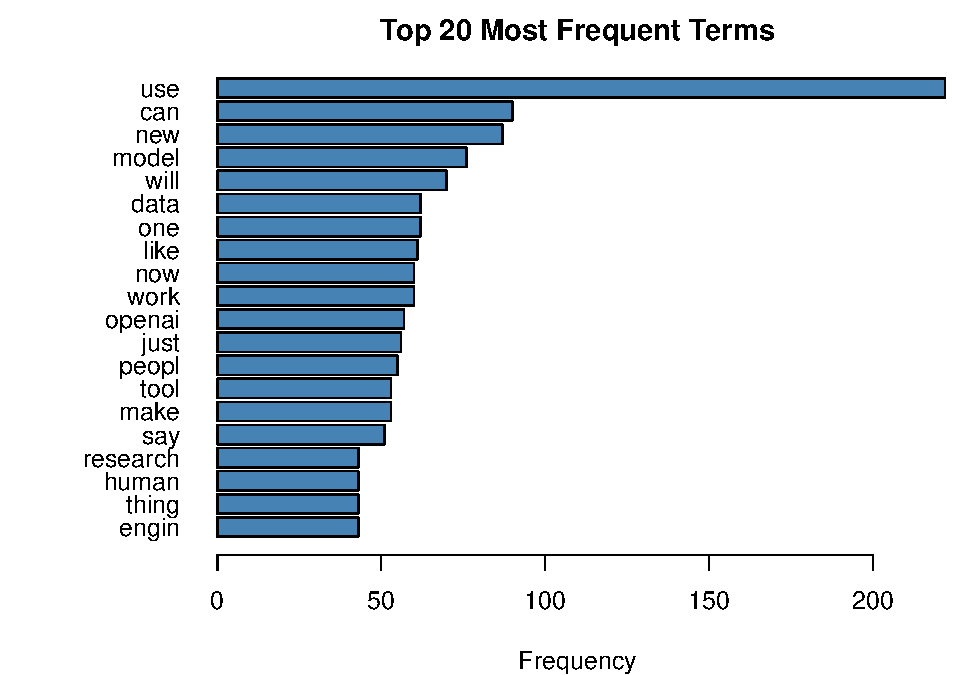
\includegraphics{Group6_analytical_report_files/figure-latex/freq-words-1} 

}

\caption{The 20 most frequent stemmed terms.}\label{fig:freq-words}
\end{figure}

\begin{Shaded}
\begin{Highlighting}[]
\FunctionTok{set.seed}\NormalTok{(}\DecValTok{3020}\NormalTok{)}
\FunctionTok{wordcloud}\NormalTok{(}\FunctionTok{names}\NormalTok{(w), w, }\AttributeTok{min.freq =} \DecValTok{10}\NormalTok{, }\AttributeTok{max.words =} \DecValTok{100}\NormalTok{,}
          \AttributeTok{random.order =} \ConstantTok{FALSE}\NormalTok{, }\AttributeTok{colors =} \FunctionTok{brewer.pal}\NormalTok{(}\DecValTok{8}\NormalTok{, }\StringTok{"Dark2"}\NormalTok{))}
\end{Highlighting}
\end{Shaded}

\begin{figure}

{\centering 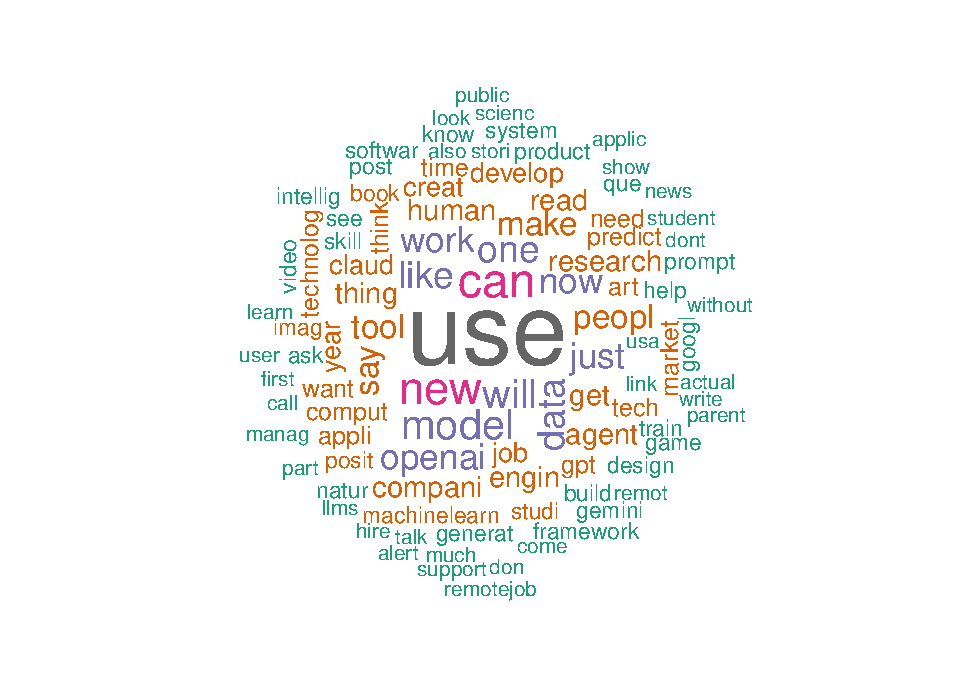
\includegraphics{Group6_analytical_report_files/figure-latex/wordcloud-1} 

}

\caption{Word cloud of terms used at least 10 times.}\label{fig:wordcloud}
\end{figure}

The most frequent term is \textbf{``use''} (222 times), followed by
\emph{can}, \emph{new}, \emph{model}, \emph{will} and \emph{data}. Terms
such as \emph{tool}, \emph{work}, \emph{research} and \emph{engin} show
that much of the discussion is about \textbf{using AI in practice},
while \emph{openai} reflects company news. Words such as \emph{peopl}
and \emph{human} point to discussion of AI's effect on people.

\subsection{Post length}\label{post-length}

\begin{Shaded}
\begin{Highlighting}[]
\NormalTok{posts}\SpecialCharTok{$}\NormalTok{post\_length }\OtherTok{=} \FunctionTok{nchar}\NormalTok{(posts}\SpecialCharTok{$}\NormalTok{text)}
\FunctionTok{summary}\NormalTok{(posts}\SpecialCharTok{$}\NormalTok{post\_length)}
\end{Highlighting}
\end{Shaded}

\begin{verbatim}
#>    Min. 1st Qu.  Median    Mean 3rd Qu.    Max. 
#>     8.0   138.0   211.0   201.4   279.5   302.0
\end{verbatim}

\begin{Shaded}
\begin{Highlighting}[]
\FunctionTok{hist}\NormalTok{(posts}\SpecialCharTok{$}\NormalTok{post\_length, }\AttributeTok{col =} \StringTok{"lightblue"}\NormalTok{, }\AttributeTok{breaks =} \DecValTok{20}\NormalTok{,}
     \AttributeTok{main =} \StringTok{"Distribution of Post Lengths"}\NormalTok{,}
     \AttributeTok{xlab =} \StringTok{"Post length (characters)"}\NormalTok{, }\AttributeTok{ylab =} \StringTok{"Number of posts"}\NormalTok{)}
\end{Highlighting}
\end{Shaded}

\begin{figure}

{\centering 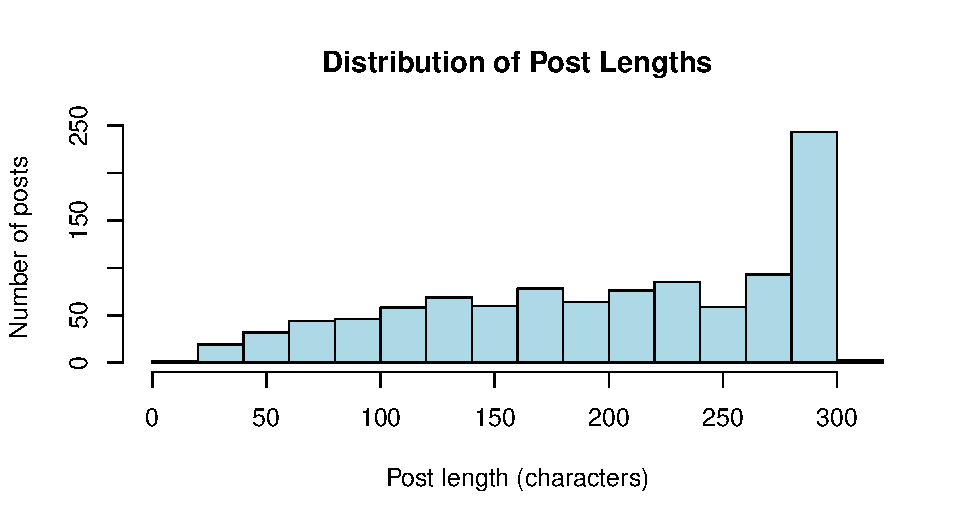
\includegraphics{Group6_analytical_report_files/figure-latex/post-length-1} 

}

\caption{Distribution of post length.}\label{fig:post-length}
\end{figure}

The median post has 211 characters. Many posts are close to Bluesky's
300-character limit, which is typical of link and headline sharing.
Short posts are often a link with a short comment.

\subsection{TF-IDF representation}\label{tf-idf-representation}

For clustering, each post is represented as a TF-IDF vector (Module 4
Part 2). TF-IDF gives more weight to terms that distinguish a post and
less weight to terms that appear everywhere.

\begin{Shaded}
\begin{Highlighting}[]
\NormalTok{N }\OtherTok{=} \FunctionTok{nrow}\NormalTok{(Bluesky.matrix)}
\NormalTok{IDF }\OtherTok{=} \FunctionTok{log}\NormalTok{(N }\SpecialCharTok{/} \FunctionTok{colSums}\NormalTok{(Bluesky.matrix }\SpecialCharTok{\textgreater{}} \DecValTok{0}\NormalTok{))}
\NormalTok{TF }\OtherTok{=} \FunctionTok{log}\NormalTok{(Bluesky.matrix }\SpecialCharTok{+} \DecValTok{1}\NormalTok{)}
\NormalTok{posts.matrix }\OtherTok{=}\NormalTok{ TF }\SpecialCharTok{\%*\%} \FunctionTok{diag}\NormalTok{(IDF)}
\FunctionTok{colnames}\NormalTok{(posts.matrix) }\OtherTok{=} \FunctionTok{colnames}\NormalTok{(Bluesky.matrix)}
\end{Highlighting}
\end{Shaded}

\section{RQ1: Topics in AI Posts
(Clustering)}\label{rq1-topics-in-ai-posts-clustering}

\subsection{Representation, distance and number of
clusters}\label{representation-distance-and-number-of-clusters}

Following Module 6:

\begin{itemize}
\tightlist
\item
  \textbf{Representation:} TF-IDF vectors, normalised to length 1 so
  long posts are not treated as different only because they contain more
  words.
\item
  \textbf{Distance:} cosine distance, which compares \emph{which} words
  are used rather than how many. It is suitable for sparse text vectors.
\item
  \textbf{Clustering:} k-means needs Euclidean distance, so
  multidimensional scaling (MDS) first places the posts in 100
  dimensions that preserve the cosine distances.
\end{itemize}

\begin{Shaded}
\begin{Highlighting}[]
\NormalTok{norm.posts.matrix }\OtherTok{=} \FunctionTok{diag}\NormalTok{(}\DecValTok{1} \SpecialCharTok{/} \FunctionTok{sqrt}\NormalTok{(}\FunctionTok{rowSums}\NormalTok{(posts.matrix}\SpecialCharTok{\^{}}\DecValTok{2}\NormalTok{))) }\SpecialCharTok{\%*\%}\NormalTok{ posts.matrix}
\NormalTok{D }\OtherTok{=} \FunctionTok{dist}\NormalTok{(norm.posts.matrix, }\AttributeTok{method =} \StringTok{"euclidean"}\NormalTok{)}\SpecialCharTok{\^{}}\DecValTok{2} \SpecialCharTok{/} \DecValTok{2}   \CommentTok{\# cosine distance}
\NormalTok{mds.posts.matrix }\OtherTok{=} \FunctionTok{cmdscale}\NormalTok{(D, }\AttributeTok{k =} \DecValTok{100}\NormalTok{)}
\end{Highlighting}
\end{Shaded}

\begin{Shaded}
\begin{Highlighting}[]
\NormalTok{n }\OtherTok{=} \DecValTok{15}
\NormalTok{SSW }\OtherTok{=} \FunctionTok{rep}\NormalTok{(}\DecValTok{0}\NormalTok{, n)}
\ControlFlowTok{for}\NormalTok{ (a }\ControlFlowTok{in} \DecValTok{1}\SpecialCharTok{:}\NormalTok{n) \{}
  \FunctionTok{set.seed}\NormalTok{(}\DecValTok{123}\NormalTok{)}
\NormalTok{  K }\OtherTok{=} \FunctionTok{kmeans}\NormalTok{(mds.posts.matrix, a, }\AttributeTok{nstart =} \DecValTok{20}\NormalTok{)}
\NormalTok{  SSW[a] }\OtherTok{=}\NormalTok{ K}\SpecialCharTok{$}\NormalTok{tot.withinss}
\NormalTok{\}}
\FunctionTok{plot}\NormalTok{(}\DecValTok{1}\SpecialCharTok{:}\NormalTok{n, SSW, }\AttributeTok{type =} \StringTok{"b"}\NormalTok{, }\AttributeTok{pch =} \DecValTok{19}\NormalTok{, }\AttributeTok{main =} \StringTok{"Elbow Method"}\NormalTok{,}
     \AttributeTok{xlab =} \StringTok{"Number of clusters (k)"}\NormalTok{, }\AttributeTok{ylab =} \StringTok{"Within{-}cluster sum of squares"}\NormalTok{)}
\FunctionTok{abline}\NormalTok{(}\AttributeTok{v =} \DecValTok{7}\NormalTok{, }\AttributeTok{col =} \StringTok{"red"}\NormalTok{, }\AttributeTok{lty =} \DecValTok{2}\NormalTok{)}
\end{Highlighting}
\end{Shaded}

\begin{figure}

{\centering 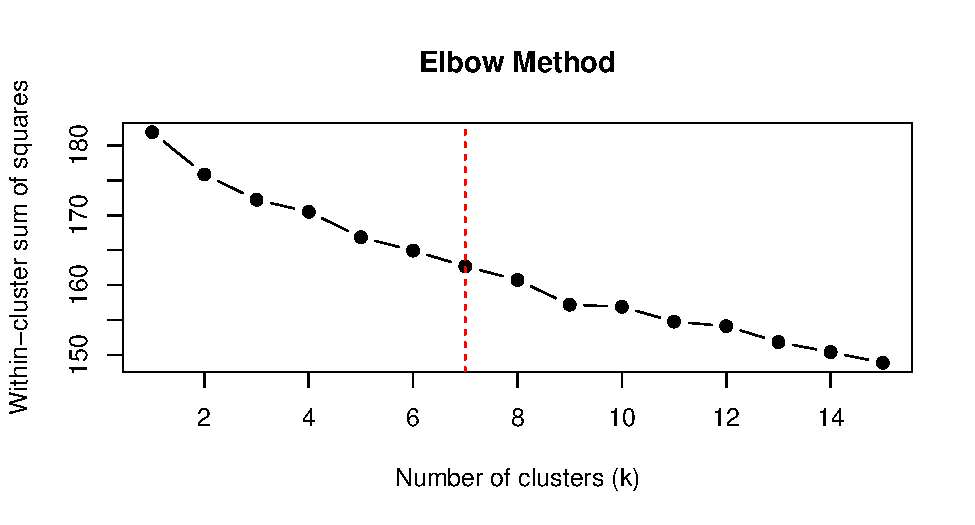
\includegraphics{Group6_analytical_report_files/figure-latex/elbow-1} 

}

\caption{Elbow method: within-cluster sum of squares for k = 1 to 15.}\label{fig:elbow}
\end{figure}

The elbow curve decreases gradually and has \textbf{no sharp elbow}.
Module 6 notes that this is common for short, sparse text. We therefore
chose \textbf{k = 7} because it was the smallest number of clusters that
separated clearly different themes (job adverts, research, polls,
Gemini, market-report spam). With fewer clusters these small themes
merged into the large general groups.

\begin{Shaded}
\begin{Highlighting}[]
\NormalTok{number.of.clusters }\OtherTok{=} \DecValTok{7}
\FunctionTok{set.seed}\NormalTok{(}\DecValTok{123}\NormalTok{)}
\NormalTok{K }\OtherTok{=} \FunctionTok{kmeans}\NormalTok{(mds.posts.matrix, number.of.clusters, }\AttributeTok{nstart =} \DecValTok{20}\NormalTok{)}
\CommentTok{\# k{-}means can give slightly different solutions on different computers}
\CommentTok{\# (numerical differences in MDS). To keep the report identical to the}
\CommentTok{\# analysis, we use the cluster labels saved by Script 03.}
\NormalTok{saved }\OtherTok{=} \FunctionTok{read.csv}\NormalTok{(}\StringTok{"data/processed/bluesky\_clustered\_posts.csv"}\NormalTok{)}
\FunctionTok{stopifnot}\NormalTok{(}\FunctionTok{all}\NormalTok{(saved}\SpecialCharTok{$}\NormalTok{uri }\SpecialCharTok{==}\NormalTok{ posts}\SpecialCharTok{$}\NormalTok{uri))}
\NormalTok{posts}\SpecialCharTok{$}\NormalTok{cluster }\OtherTok{=}\NormalTok{ saved}\SpecialCharTok{$}\NormalTok{cluster}
\FunctionTok{table}\NormalTok{(posts}\SpecialCharTok{$}\NormalTok{cluster)}
\end{Highlighting}
\end{Shaded}

\begin{verbatim}
#> 
#>   1   2   3   4   5   6   7 
#>  18 113   7  14 261 589  29
\end{verbatim}

\begin{Shaded}
\begin{Highlighting}[]
\CommentTok{\# Proportion of total variation explained by the saved clusters.}
\NormalTok{centres }\OtherTok{=} \FunctionTok{apply}\NormalTok{(mds.posts.matrix, }\DecValTok{2}\NormalTok{, }\ControlFlowTok{function}\NormalTok{(v) }\FunctionTok{tapply}\NormalTok{(v, posts}\SpecialCharTok{$}\NormalTok{cluster, mean))}
\NormalTok{within.ss }\OtherTok{=} \FunctionTok{sum}\NormalTok{((mds.posts.matrix }\SpecialCharTok{{-}}\NormalTok{ centres[posts}\SpecialCharTok{$}\NormalTok{cluster, ])}\SpecialCharTok{\^{}}\DecValTok{2}\NormalTok{)}
\NormalTok{total.ss }\OtherTok{=} \FunctionTok{sum}\NormalTok{(}\FunctionTok{scale}\NormalTok{(mds.posts.matrix, }\AttributeTok{scale =} \ConstantTok{FALSE}\NormalTok{)}\SpecialCharTok{\^{}}\DecValTok{2}\NormalTok{)}
\NormalTok{explained }\OtherTok{=} \DecValTok{1} \SpecialCharTok{{-}}\NormalTok{ within.ss }\SpecialCharTok{/}\NormalTok{ total.ss}
\end{Highlighting}
\end{Shaded}

\subsection{Cluster themes}\label{cluster-themes}

For each cluster we averaged the TF-IDF weight of every term over the
cluster's posts. The highest averages describe the cluster (Module 6).
We also read example posts to name each theme.

\begin{Shaded}
\begin{Highlighting}[]
\NormalTok{cluster.names }\OtherTok{=} \FunctionTok{c}\NormalTok{(}\StringTok{"Remote ML job adverts (bots)"}\NormalTok{,}
                  \StringTok{"AI research, books and academia"}\NormalTok{,}
                  \StringTok{"AP{-}NORC poll: AI developing too fast"}\NormalTok{,}
                  \StringTok{"Google Gemini, Claude and enterprise agents"}\NormalTok{,}
                  \StringTok{"Personal opinions on using AI"}\NormalTok{,}
                  \StringTok{"General AI news and link sharing"}\NormalTok{,}
                  \StringTok{"Market{-}report spam"}\NormalTok{)}

\CommentTok{\# One fixed colour per cluster, used in every plot so colours always match.}
\NormalTok{cluster.colours }\OtherTok{=} \FunctionTok{c}\NormalTok{(}\StringTok{"\#9AA0A6"}\NormalTok{, }\StringTok{"\#7B5EA7"}\NormalTok{, }\StringTok{"\#B8BCC2"}\NormalTok{, }\StringTok{"\#E0A030"}\NormalTok{,}
                    \StringTok{"\#1B9E77"}\NormalTok{, }\StringTok{"\#2C6FB7"}\NormalTok{, }\StringTok{"\#5F6368"}\NormalTok{)}

\NormalTok{top.terms }\OtherTok{=} \FunctionTok{rep}\NormalTok{(}\StringTok{""}\NormalTok{, number.of.clusters)}
\ControlFlowTok{for}\NormalTok{ (a }\ControlFlowTok{in} \DecValTok{1}\SpecialCharTok{:}\NormalTok{number.of.clusters) \{}
\NormalTok{  clusterTermWeight }\OtherTok{=} \FunctionTok{colMeans}\NormalTok{(posts.matrix[posts}\SpecialCharTok{$}\NormalTok{cluster }\SpecialCharTok{==}\NormalTok{ a, , }\AttributeTok{drop =} \ConstantTok{FALSE}\NormalTok{])}
\NormalTok{  top.terms[a] }\OtherTok{=} \FunctionTok{paste}\NormalTok{(}\FunctionTok{names}\NormalTok{(}\FunctionTok{sort}\NormalTok{(clusterTermWeight, }\AttributeTok{decreasing =} \ConstantTok{TRUE}\NormalTok{))[}\DecValTok{1}\SpecialCharTok{:}\DecValTok{6}\NormalTok{],}
                       \AttributeTok{collapse =} \StringTok{", "}\NormalTok{)}
\NormalTok{\}}

\NormalTok{cluster.table }\OtherTok{=} \FunctionTok{data.frame}\NormalTok{(}\AttributeTok{Cluster =} \DecValTok{1}\SpecialCharTok{:}\NormalTok{number.of.clusters,}
                           \AttributeTok{Posts =} \FunctionTok{as.vector}\NormalTok{(}\FunctionTok{table}\NormalTok{(posts}\SpecialCharTok{$}\NormalTok{cluster)),}
                           \AttributeTok{Theme =}\NormalTok{ cluster.names,}
                           \AttributeTok{Top\_terms =}\NormalTok{ top.terms)}
\NormalTok{knitr}\SpecialCharTok{::}\FunctionTok{kable}\NormalTok{(cluster.table, }\AttributeTok{caption =} \StringTok{"Cluster sizes, themes and top TF{-}IDF terms."}\NormalTok{)}
\end{Highlighting}
\end{Shaded}

\begin{longtable}[]{@{}
  >{\raggedleft\arraybackslash}p{(\linewidth - 6\tabcolsep) * \real{0.0721}}
  >{\raggedleft\arraybackslash}p{(\linewidth - 6\tabcolsep) * \real{0.0541}}
  >{\raggedright\arraybackslash}p{(\linewidth - 6\tabcolsep) * \real{0.3964}}
  >{\raggedright\arraybackslash}p{(\linewidth - 6\tabcolsep) * \real{0.4775}}@{}}
\caption{Cluster sizes, themes and top TF-IDF terms.}\tabularnewline
\toprule\noalign{}
\begin{minipage}[b]{\linewidth}\raggedleft
Cluster
\end{minipage} & \begin{minipage}[b]{\linewidth}\raggedleft
Posts
\end{minipage} & \begin{minipage}[b]{\linewidth}\raggedright
Theme
\end{minipage} & \begin{minipage}[b]{\linewidth}\raggedright
Top\_terms
\end{minipage} \\
\midrule\noalign{}
\endfirsthead
\toprule\noalign{}
\begin{minipage}[b]{\linewidth}\raggedleft
Cluster
\end{minipage} & \begin{minipage}[b]{\linewidth}\raggedleft
Posts
\end{minipage} & \begin{minipage}[b]{\linewidth}\raggedright
Theme
\end{minipage} & \begin{minipage}[b]{\linewidth}\raggedright
Top\_terms
\end{minipage} \\
\midrule\noalign{}
\endhead
\bottomrule\noalign{}
\endlastfoot
1 & 18 & Remote ML job adverts (bots) & remotejob, remotework, remot,
locat, alert, categori \\
2 & 113 & AI research, books and academia & model, research, book,
sinkan, springer, natur \\
3 & 7 & AP-NORC poll: AI developing too fast & apnorc, fast, american,
poll, find, develop \\
4 & 14 & Google Gemini, Claude and enterprise agents & gemini, claud,
googl, geminiai, introduc, work \\
5 & 261 & Personal opinions on using AI & can, use, just, will, peopl,
like \\
6 & 589 & General AI news and link sharing & use, agent, data, new, que,
read \\
7 & 29 & Market-report spam & gpt, intellig, size, growth, openai,
interact \\
\end{longtable}

\begin{Shaded}
\begin{Highlighting}[]
\CommentTok{\# One example post per cluster (shortened, non{-}English characters removed).}
\ControlFlowTok{for}\NormalTok{ (a }\ControlFlowTok{in} \DecValTok{1}\SpecialCharTok{:}\NormalTok{number.of.clusters) \{}
\NormalTok{  example }\OtherTok{=}\NormalTok{ posts}\SpecialCharTok{$}\NormalTok{text[posts}\SpecialCharTok{$}\NormalTok{cluster }\SpecialCharTok{==}\NormalTok{ a][}\DecValTok{1}\NormalTok{]}
\NormalTok{  example }\OtherTok{=} \FunctionTok{iconv}\NormalTok{(}\FunctionTok{gsub}\NormalTok{(}\StringTok{"}\SpecialCharTok{\textbackslash{}\textbackslash{}}\StringTok{s+"}\NormalTok{, }\StringTok{" "}\NormalTok{, example), }\AttributeTok{to =} \StringTok{"ASCII"}\NormalTok{, }\AttributeTok{sub =} \StringTok{""}\NormalTok{)}
  \FunctionTok{cat}\NormalTok{(}\StringTok{"Cluster"}\NormalTok{, a, }\StringTok{":"}\NormalTok{, }\FunctionTok{substr}\NormalTok{(example, }\DecValTok{1}\NormalTok{, }\DecValTok{85}\NormalTok{), }\StringTok{"}\SpecialCharTok{\textbackslash{}n}\StringTok{"}\NormalTok{)}
\NormalTok{\}}
\end{Highlighting}
\end{Shaded}

\begin{verbatim}
#> Cluster 1 :  New Remote Job Alert!  Position: Resident Engineer  Company: Extreme Networks  Locat 
#> Cluster 2 : The evening featured Perimeter researchers Sabrina Pasterski and Tim Hsieh, who are e 
#> Cluster 3 : Most Americans think artificial intelligence is developing too fast, a new AP-NORC po 
#> Cluster 4 : Google Cloud introduces Gemini agent to change enterprise work ->SiliconANGLE | More  
#> Cluster 5 : Worthy of a watch. An argument to slow down or pause the development of AGI, which ca 
#> Cluster 6 : www.socialmediatoday.com/news/ai-favo... AI favors brands with an active social media 
#> Cluster 7 : Robotics System Integration Market Size, Growth Report 2035 www.marketresearchfuture.
\end{verbatim}

\begin{Shaded}
\begin{Highlighting}[]
\NormalTok{mds2.posts.matrix }\OtherTok{=} \FunctionTok{cmdscale}\NormalTok{(D, }\AttributeTok{k =} \DecValTok{2}\NormalTok{)}

\FunctionTok{plot}\NormalTok{(mds2.posts.matrix, }\AttributeTok{col =}\NormalTok{ cluster.colours[posts}\SpecialCharTok{$}\NormalTok{cluster], }\AttributeTok{pch =} \DecValTok{19}\NormalTok{, }\AttributeTok{cex =} \FloatTok{0.6}\NormalTok{,}
     \AttributeTok{main =} \StringTok{"AI Discussion Clusters (2D MDS)"}\NormalTok{,}
     \AttributeTok{xlab =} \StringTok{"MDS dimension 1"}\NormalTok{, }\AttributeTok{ylab =} \StringTok{"MDS dimension 2"}\NormalTok{)}
\CommentTok{\# Legend in the empty top{-}left corner so it does not cover the posts.}
\FunctionTok{legend}\NormalTok{(}\StringTok{"topleft"}\NormalTok{, }\AttributeTok{legend =} \FunctionTok{paste}\NormalTok{(}\DecValTok{1}\SpecialCharTok{:}\DecValTok{7}\NormalTok{, cluster.names), }\AttributeTok{col =}\NormalTok{ cluster.colours,}
       \AttributeTok{pch =} \DecValTok{19}\NormalTok{, }\AttributeTok{cex =} \FloatTok{0.7}\NormalTok{, }\AttributeTok{bty =} \StringTok{"n"}\NormalTok{)}
\end{Highlighting}
\end{Shaded}

\begin{figure}

{\centering 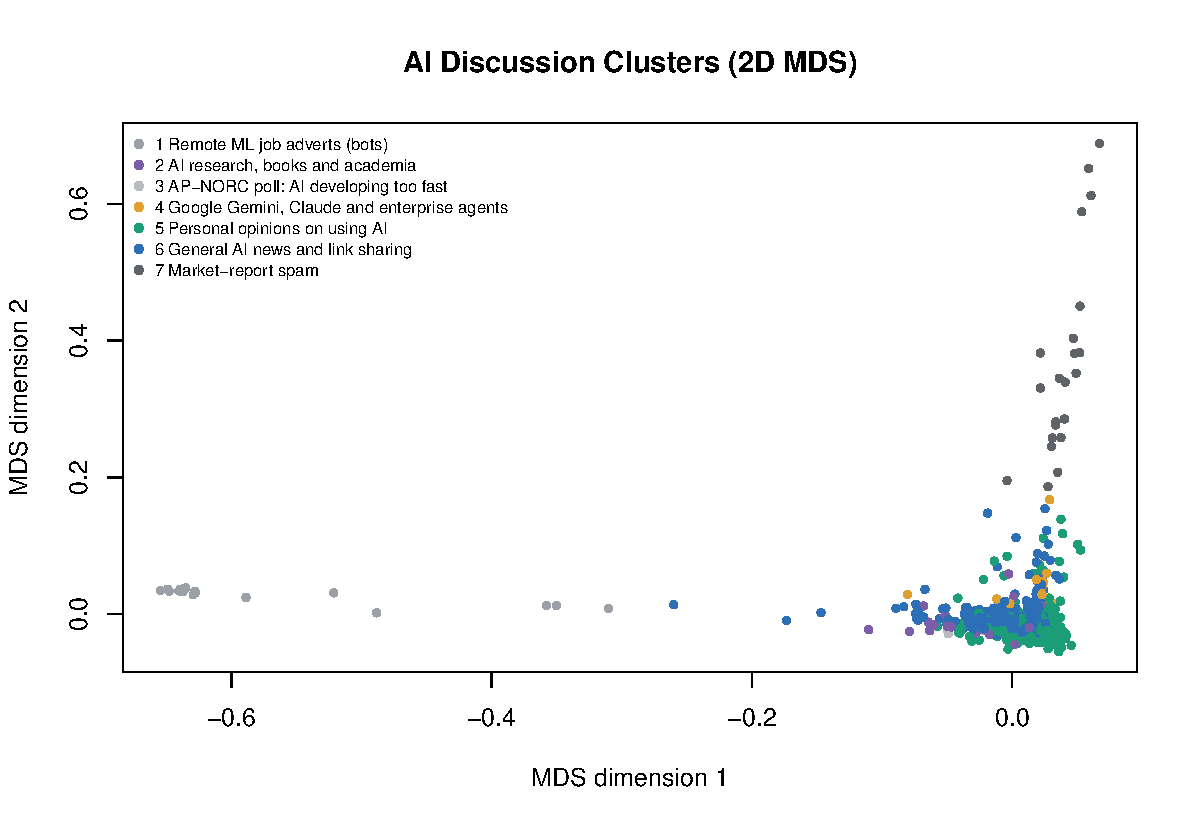
\includegraphics{Group6_analytical_report_files/figure-latex/mds-plot-1} 

}

\caption{Posts in two MDS dimensions, coloured by cluster.}\label{fig:mds-plot}
\end{figure}

\subsection{Interpretation}\label{interpretation}

\begin{itemize}
\tightlist
\item
  Two large clusters dominate. \textbf{Cluster 6} (589 posts) is general
  AI news and link sharing about agents, data, OpenAI and policy.
  \textbf{Cluster 5} (261 posts) contains personal opinions about using
  AI (\emph{can, use, just, people, think, tool}).
\item
  \textbf{Cluster 2} groups research and academic content, including
  automated new-book listings.
\item
  Three small clusters are \textbf{automated or repeated content}:
  remote-job bots (1), one AP-NORC poll story posted many times (3) and
  market-report spam (7). Together with the 87 duplicate texts removed
  during cleaning, this shows that a noticeable part of ``AI
  discussion'' on Bluesky is not personal conversation.
\item
  In the 2D MDS plot, the job-advert bots (Cluster 1) and market-report
  spam (Cluster 7) form clearly separate groups, while the other
  clusters overlap near the centre. Two dimensions cannot show all the
  differences that k-means found in 100 dimensions, and the large
  clusters share common vocabulary, so their boundary is less sharp. The
  k-means clusters explain only 10.6\% of the total variation, so the
  themes are useful descriptions rather than strict categories.
\end{itemize}

\subsection{Do the clusters simply repeat the search
terms?}\label{do-the-clusters-simply-repeat-the-search-terms}

Every post was found by one of four search terms, so a concern is that
the clusters only reproduce those terms. A chi-squared test of
independence (Module 9) compares the search term of each post with its
cluster. Some cells are small, so the p-value is simulated.

\begin{itemize}
\tightlist
\item
  \textbf{H0:} cluster membership is independent of the search term
\item
  \textbf{HA:} cluster membership depends on the search term
\end{itemize}

\begin{Shaded}
\begin{Highlighting}[]
\NormalTok{keyword.table }\OtherTok{=} \FunctionTok{table}\NormalTok{(posts}\SpecialCharTok{$}\NormalTok{search\_keyword, posts}\SpecialCharTok{$}\NormalTok{cluster)}
\NormalTok{keyword.table}
\end{Highlighting}
\end{Shaded}

\begin{verbatim}
#>                          
#>                             1   2   3   4   5   6   7
#>   artificial intelligence   0  28   7   1  46 168   6
#>   ChatGPT                   0   6   0  10  80 135  23
#>   generative AI             0  11   0   1  95 141   0
#>   machine learning         18  68   0   2  40 145   0
\end{verbatim}

\begin{Shaded}
\begin{Highlighting}[]
\FunctionTok{set.seed}\NormalTok{(}\DecValTok{123}\NormalTok{)}
\FunctionTok{chisq.test}\NormalTok{(keyword.table, }\AttributeTok{simulate.p.value =} \ConstantTok{TRUE}\NormalTok{, }\AttributeTok{B =} \DecValTok{2000}\NormalTok{)}
\end{Highlighting}
\end{Shaded}

\begin{verbatim}
#> 
#>  Pearson's Chi-squared test with simulated p-value (based on 2000
#>  replicates)
#> 
#> data:  keyword.table
#> X-squared = 255.89, df = NA, p-value = 0.0004998
\end{verbatim}

The test rejects H0 (p \textless{} 0.001): topics are related to the
search term (for example, the research cluster comes mostly from
\emph{machine learning} and \emph{artificial intelligence}). However,
the two largest clusters contain posts from all four search terms, so
the clusters capture themes that cut across the queries rather than
simply repeating them.

\section{RQ2: Does Engagement Differ Between
Topics?}\label{rq2-does-engagement-differ-between-topics}

\subsection{Hypotheses and choice of
test}\label{hypotheses-and-choice-of-test}

Engagement of a post = likes + reposts + replies. The two largest
clusters represent two different kinds of AI posts: \textbf{news/link
sharing (Cluster 6)} and \textbf{personal opinion (Cluster 5)}. These
two clusters were chosen \textbf{before} looking at engagement, because
they are the two largest clusters and together contain most posts. We
test whether their mean engagement differs:

\begin{itemize}
\tightlist
\item
  \textbf{H0:} mean engagement of news posts = mean engagement of
  opinion posts
\item
  \textbf{HA:} mean engagement of news posts \(\neq\) mean engagement of
  opinion posts (two-sided, \(\alpha = 0.05\))
\end{itemize}

We use the \textbf{randomisation (permutation) test for a difference in
means} from Module 10. Engagement is very skewed (most posts have 0),
and the randomisation test does not assume a normal distribution. A
Welch t-test is reported for comparison.

\begin{Shaded}
\begin{Highlighting}[]
\NormalTok{posts}\SpecialCharTok{$}\NormalTok{engagement }\OtherTok{=}\NormalTok{ posts}\SpecialCharTok{$}\NormalTok{like\_count }\SpecialCharTok{+}\NormalTok{ posts}\SpecialCharTok{$}\NormalTok{repost\_count }\SpecialCharTok{+}\NormalTok{ posts}\SpecialCharTok{$}\NormalTok{reply\_count}
\FunctionTok{summary}\NormalTok{(posts}\SpecialCharTok{$}\NormalTok{engagement)}
\end{Highlighting}
\end{Shaded}

\begin{verbatim}
#>    Min. 1st Qu.  Median    Mean 3rd Qu.    Max. 
#>   0.000   0.000   0.000   2.646   2.000 265.000
\end{verbatim}

\begin{Shaded}
\begin{Highlighting}[]
\NormalTok{groupA }\OtherTok{=}\NormalTok{ posts}\SpecialCharTok{$}\NormalTok{engagement[posts}\SpecialCharTok{$}\NormalTok{cluster }\SpecialCharTok{==} \DecValTok{6}\NormalTok{]   }\CommentTok{\# news}
\NormalTok{groupB }\OtherTok{=}\NormalTok{ posts}\SpecialCharTok{$}\NormalTok{engagement[posts}\SpecialCharTok{$}\NormalTok{cluster }\SpecialCharTok{==} \DecValTok{5}\NormalTok{]   }\CommentTok{\# opinion}
\FunctionTok{c}\NormalTok{(}\AttributeTok{n\_news =} \FunctionTok{length}\NormalTok{(groupA), }\AttributeTok{n\_opinion =} \FunctionTok{length}\NormalTok{(groupB))}
\end{Highlighting}
\end{Shaded}

\begin{verbatim}
#>    n_news n_opinion 
#>       589       261
\end{verbatim}

\begin{Shaded}
\begin{Highlighting}[]
\FunctionTok{c}\NormalTok{(}\AttributeTok{mean\_news =} \FunctionTok{mean}\NormalTok{(groupA), }\AttributeTok{mean\_opinion =} \FunctionTok{mean}\NormalTok{(groupB))}
\end{Highlighting}
\end{Shaded}

\begin{verbatim}
#>    mean_news mean_opinion 
#>     2.432937     4.298851
\end{verbatim}

\begin{Shaded}
\begin{Highlighting}[]
\NormalTok{meanDiff }\OtherTok{=} \FunctionTok{mean}\NormalTok{(groupB) }\SpecialCharTok{{-}} \FunctionTok{mean}\NormalTok{(groupA)}
\NormalTok{meanDiff}
\end{Highlighting}
\end{Shaded}

\begin{verbatim}
#> [1] 1.865913
\end{verbatim}

\begin{Shaded}
\begin{Highlighting}[]
\NormalTok{shuffleMean }\OtherTok{=} \ControlFlowTok{function}\NormalTok{(groupA, groupB) \{}
\NormalTok{  combined }\OtherTok{=} \FunctionTok{c}\NormalTok{(groupA, groupB)}
\NormalTok{  chosen }\OtherTok{=} \FunctionTok{sample}\NormalTok{(}\FunctionTok{length}\NormalTok{(combined), }\AttributeTok{size =} \FunctionTok{length}\NormalTok{(groupA), }\AttributeTok{replace =} \ConstantTok{FALSE}\NormalTok{)}
  \FunctionTok{mean}\NormalTok{(combined[}\SpecialCharTok{{-}}\NormalTok{chosen]) }\SpecialCharTok{{-}} \FunctionTok{mean}\NormalTok{(combined[chosen])}
\NormalTok{\}}
\FunctionTok{set.seed}\NormalTok{(}\DecValTok{123}\NormalTok{)}
\NormalTok{randDist }\OtherTok{=} \FunctionTok{replicate}\NormalTok{(}\DecValTok{1000}\NormalTok{, }\FunctionTok{shuffleMean}\NormalTok{(groupA, groupB))}
\FunctionTok{hist}\NormalTok{(randDist, }\AttributeTok{col =} \StringTok{"lightblue"}\NormalTok{, }\AttributeTok{main =} \StringTok{"Randomisation Distribution"}\NormalTok{,}
     \AttributeTok{xlab =} \StringTok{"Difference in mean engagement (opinion {-} news)"}\NormalTok{)}
\FunctionTok{abline}\NormalTok{(}\AttributeTok{v =}\NormalTok{ meanDiff, }\AttributeTok{col =} \StringTok{"red"}\NormalTok{, }\AttributeTok{lwd =} \DecValTok{2}\NormalTok{)}
\end{Highlighting}
\end{Shaded}

\begin{figure}

{\centering 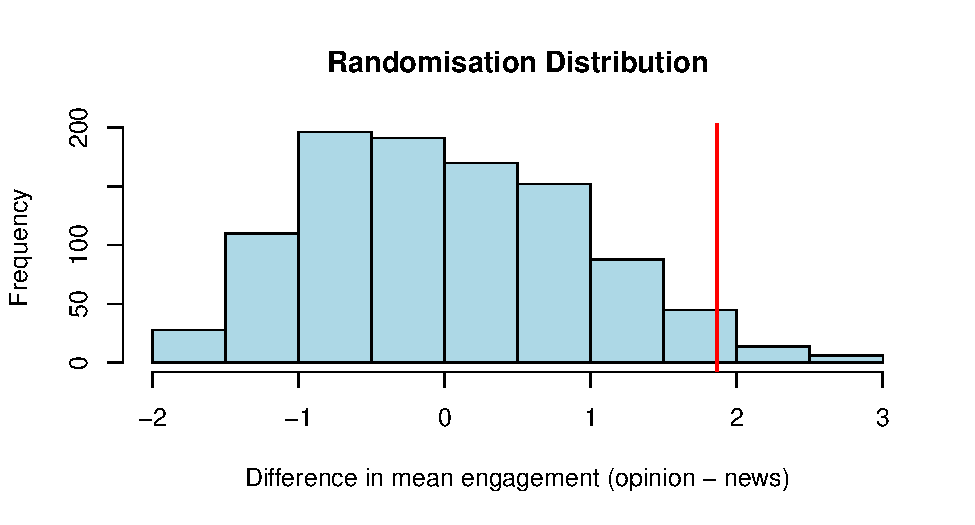
\includegraphics{Group6_analytical_report_files/figure-latex/randomisation-1} 

}

\caption{Randomisation distribution of the difference in means under H0; the red line is the observed difference.}\label{fig:randomisation}
\end{figure}

\begin{Shaded}
\begin{Highlighting}[]
\NormalTok{pVal }\OtherTok{=} \FunctionTok{mean}\NormalTok{(}\FunctionTok{abs}\NormalTok{(randDist) }\SpecialCharTok{\textgreater{}} \FunctionTok{abs}\NormalTok{(meanDiff))}
\NormalTok{pVal}
\end{Highlighting}
\end{Shaded}

\begin{verbatim}
#> [1] 0.032
\end{verbatim}

\begin{Shaded}
\begin{Highlighting}[]
\NormalTok{tt }\OtherTok{=} \FunctionTok{t.test}\NormalTok{(groupA, groupB)}
\NormalTok{tt}\SpecialCharTok{$}\NormalTok{p.value}
\end{Highlighting}
\end{Shaded}

\begin{verbatim}
#> [1] 0.04591426
\end{verbatim}

\subsection{Comparing all seven
topics}\label{comparing-all-seven-topics}

To check RQ2 across \textbf{all} topics, a one-way ANOVA (the
\texttt{aov()} function used in Module 10) compares the mean engagement
of the seven clusters. Here H0 is that all clusters have the same mean
engagement.

\begin{Shaded}
\begin{Highlighting}[]
\CommentTok{\# Mean engagement of each cluster.}
\NormalTok{cluster.means }\OtherTok{=} \FunctionTok{rep}\NormalTok{(}\DecValTok{0}\NormalTok{, number.of.clusters)}
\ControlFlowTok{for}\NormalTok{ (a }\ControlFlowTok{in} \DecValTok{1}\SpecialCharTok{:}\NormalTok{number.of.clusters) \{}
\NormalTok{  cluster.means[a] }\OtherTok{=} \FunctionTok{mean}\NormalTok{(posts}\SpecialCharTok{$}\NormalTok{engagement[posts}\SpecialCharTok{$}\NormalTok{cluster }\SpecialCharTok{==}\NormalTok{ a])}
\NormalTok{\}}
\FunctionTok{round}\NormalTok{(cluster.means, }\DecValTok{2}\NormalTok{)}
\end{Highlighting}
\end{Shaded}

\begin{verbatim}
#> [1] 0.00 1.42 0.43 0.29 4.30 2.43 0.17
\end{verbatim}

\begin{Shaded}
\begin{Highlighting}[]
\FunctionTok{barplot}\NormalTok{(cluster.means, }\AttributeTok{names.arg =} \DecValTok{1}\SpecialCharTok{:}\DecValTok{7}\NormalTok{,}
        \AttributeTok{col =} \FunctionTok{c}\NormalTok{(}\StringTok{"grey"}\NormalTok{, }\StringTok{"grey"}\NormalTok{, }\StringTok{"grey"}\NormalTok{, }\StringTok{"grey"}\NormalTok{, }\StringTok{"lightgreen"}\NormalTok{, }\StringTok{"lightblue"}\NormalTok{, }\StringTok{"grey"}\NormalTok{),}
        \AttributeTok{main =} \StringTok{"Mean Engagement by Topic Cluster"}\NormalTok{,}
        \AttributeTok{xlab =} \StringTok{"Cluster"}\NormalTok{, }\AttributeTok{ylab =} \StringTok{"Mean likes + reposts + replies"}\NormalTok{)}
\end{Highlighting}
\end{Shaded}

\begin{figure}

{\centering 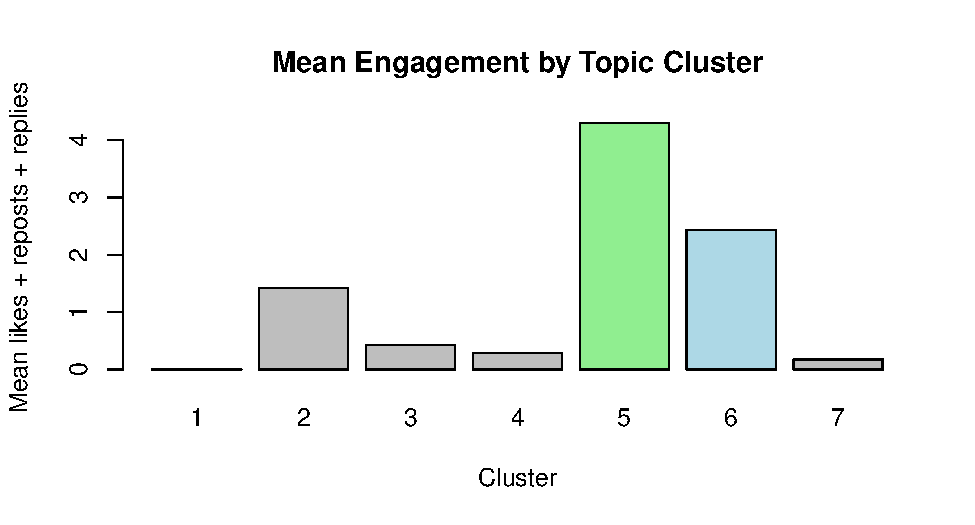
\includegraphics{Group6_analytical_report_files/figure-latex/anova-1} 

}

\caption{Mean engagement of each topic cluster; the two tested clusters are highlighted.}\label{fig:anova}
\end{figure}

\begin{Shaded}
\begin{Highlighting}[]
\CommentTok{\# factor() tells R that the cluster numbers are group labels.}
\NormalTok{model }\OtherTok{=} \FunctionTok{aov}\NormalTok{(engagement }\SpecialCharTok{\textasciitilde{}} \FunctionTok{factor}\NormalTok{(cluster), }\AttributeTok{data =}\NormalTok{ posts)}
\FunctionTok{summary}\NormalTok{(model)}
\end{Highlighting}
\end{Shaded}

\begin{verbatim}
#>                   Df Sum Sq Mean Sq F value Pr(>F)
#> factor(cluster)    6   1324   220.7   1.694  0.119
#> Residuals       1024 133406   130.3
\end{verbatim}

\begin{Shaded}
\begin{Highlighting}[]
\NormalTok{anova.p }\OtherTok{=} \FunctionTok{summary}\NormalTok{(model)[[}\DecValTok{1}\NormalTok{]][[}\StringTok{"Pr(\textgreater{}F)"}\NormalTok{]][}\DecValTok{1}\NormalTok{]}
\end{Highlighting}
\end{Shaded}

\subsection{Interpretation}\label{interpretation-1}

\begin{itemize}
\tightlist
\item
  Opinion posts received on average \textbf{4.3} engagements, compared
  with \textbf{2.43} for news posts. The difference is 1.87.
\item
  The randomisation p-value is \textbf{0.032} and the t-test p-value is
  \textbf{0.046}. Both are below 0.05, so \textbf{we reject H0}:
  personal opinion posts about AI attract more engagement than news and
  link-sharing posts. The t-test p-value is close to 0.05 and the median
  engagement of both groups is 0, so the difference in means is driven
  by a smaller number of posts with high engagement. The evidence is
  therefore moderate.
\item
  The ANOVA across all seven clusters is \textbf{not significant} (p =
  0.119). The engagement distribution is very skewed and several
  clusters are small, which may limit the power of this test. However,
  the automated clusters (1, 3, 7) have mean engagement close to zero,
  which supports the RQ1 finding that this content is largely ignored by
  users.
\end{itemize}

\section{RQ3: Follow Network of AI Post
Authors}\label{rq3-follow-network-of-ai-post-authors}

\subsection{Network definition}\label{network-definition}

\begin{itemize}
\tightlist
\item
  \textbf{Node:} an author of at least one AI post in the cleaned data.
\item
  \textbf{Edge A → B:} author A follows author B, taken from the
  \texttt{get\_follows()} data.
\item
  The graph is \textbf{directed} because following is one-way: A can
  follow B without B following A.
\end{itemize}

Most collected follows point to accounts that did not post about AI in
our sample, so only follows \textbf{between} AI-post authors are kept.
This makes the network directly about the AI discussion community.

\begin{Shaded}
\begin{Highlighting}[]
\FunctionTok{library}\NormalTok{(igraph)}
\NormalTok{edges }\OtherTok{=} \FunctionTok{read.csv}\NormalTok{(}\StringTok{"data/raw/bluesky\_follow\_edges.csv"}\NormalTok{)}
\NormalTok{ai\_users }\OtherTok{=} \FunctionTok{unique}\NormalTok{(posts}\SpecialCharTok{$}\NormalTok{author\_handle)}

\NormalTok{el }\OtherTok{=} \FunctionTok{as.matrix}\NormalTok{(edges[, }\FunctionTok{c}\NormalTok{(}\StringTok{"from"}\NormalTok{, }\StringTok{"to"}\NormalTok{)])}
\NormalTok{el }\OtherTok{=} \FunctionTok{unique}\NormalTok{(el)}
\NormalTok{el }\OtherTok{=}\NormalTok{ el[el[, }\StringTok{"from"}\NormalTok{] }\SpecialCharTok{!=}\NormalTok{ el[, }\StringTok{"to"}\NormalTok{], ]}
\NormalTok{el }\OtherTok{=}\NormalTok{ el[el[, }\StringTok{"from"}\NormalTok{] }\SpecialCharTok{\%in\%}\NormalTok{ ai\_users }\SpecialCharTok{\&}\NormalTok{ el[, }\StringTok{"to"}\NormalTok{] }\SpecialCharTok{\%in\%}\NormalTok{ ai\_users, ]}

\NormalTok{g }\OtherTok{=} \FunctionTok{graph\_from\_edgelist}\NormalTok{(el, }\AttributeTok{directed =} \ConstantTok{TRUE}\NormalTok{)}
\NormalTok{comp }\OtherTok{=} \FunctionTok{components}\NormalTok{(g, }\AttributeTok{mode =} \StringTok{"weak"}\NormalTok{)}
\end{Highlighting}
\end{Shaded}

\subsection{Network properties}\label{network-properties}

\begin{Shaded}
\begin{Highlighting}[]
\NormalTok{network.summary }\OtherTok{=} \FunctionTok{data.frame}\NormalTok{(}
  \AttributeTok{Measure =} \FunctionTok{c}\NormalTok{(}\StringTok{"AI{-}post authors"}\NormalTok{, }\StringTok{"Authors with at least one tie (nodes)"}\NormalTok{,}
              \StringTok{"Authors with no tie (not in graph)"}\NormalTok{, }\StringTok{"Edges (follows)"}\NormalTok{,}
              \StringTok{"Density"}\NormalTok{, }\StringTok{"Weakly connected components"}\NormalTok{,}
              \StringTok{"Size of largest component"}\NormalTok{),}
  \AttributeTok{Value =} \FunctionTok{c}\NormalTok{(}\FunctionTok{length}\NormalTok{(ai\_users), }\FunctionTok{vcount}\NormalTok{(g), }\FunctionTok{length}\NormalTok{(ai\_users) }\SpecialCharTok{{-}} \FunctionTok{vcount}\NormalTok{(g),}
            \FunctionTok{ecount}\NormalTok{(g), }\FunctionTok{round}\NormalTok{(}\FunctionTok{edge\_density}\NormalTok{(g), }\DecValTok{4}\NormalTok{), comp}\SpecialCharTok{$}\NormalTok{no, }\FunctionTok{max}\NormalTok{(comp}\SpecialCharTok{$}\NormalTok{csize)))}
\NormalTok{knitr}\SpecialCharTok{::}\FunctionTok{kable}\NormalTok{(network.summary, }\AttributeTok{caption =} \StringTok{"Properties of the AI{-}author follow network."}\NormalTok{)}
\end{Highlighting}
\end{Shaded}

\begin{longtable}[]{@{}lr@{}}
\caption{Properties of the AI-author follow network.}\tabularnewline
\toprule\noalign{}
Measure & Value \\
\midrule\noalign{}
\endfirsthead
\toprule\noalign{}
Measure & Value \\
\midrule\noalign{}
\endhead
\bottomrule\noalign{}
\endlastfoot
AI-post authors & 803.0000 \\
Authors with at least one tie (nodes) & 340.0000 \\
Authors with no tie (not in graph) & 463.0000 \\
Edges (follows) & 480.0000 \\
Density & 0.0042 \\
Weakly connected components & 18.0000 \\
Size of largest component & 294.0000 \\
\end{longtable}

\begin{Shaded}
\begin{Highlighting}[]
\FunctionTok{plot}\NormalTok{(}\FunctionTok{degree\_distribution}\NormalTok{(g), }\AttributeTok{type =} \StringTok{"h"}\NormalTok{, }\AttributeTok{xlab =} \StringTok{"Degree"}\NormalTok{, }\AttributeTok{ylab =} \StringTok{"Proportion"}\NormalTok{,}
     \AttributeTok{main =} \StringTok{"Degree Distribution of the AI Author Network"}\NormalTok{)}
\end{Highlighting}
\end{Shaded}

\begin{figure}

{\centering 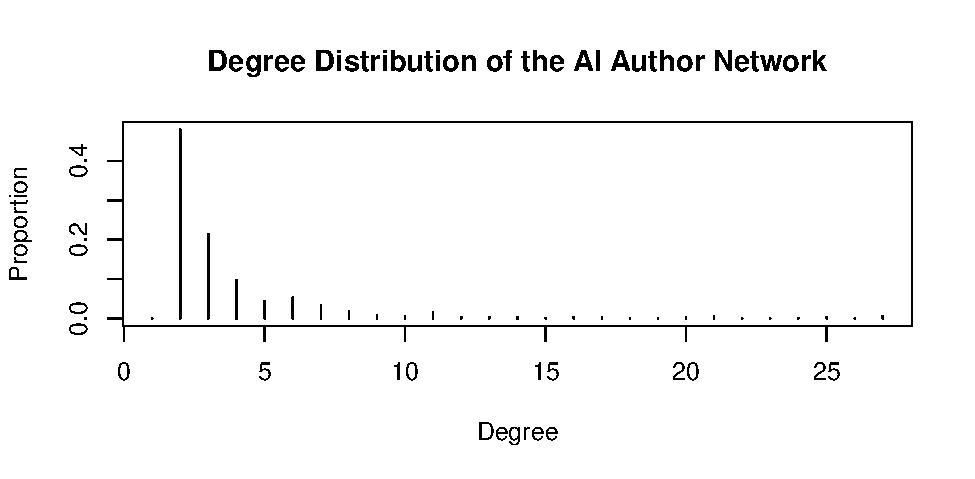
\includegraphics{Group6_analytical_report_files/figure-latex/degree-dist-1} 

}

\caption{Degree distribution of the network.}\label{fig:degree-dist}
\end{figure}

Among the connected authors, the network is \textbf{sparse} (density
0.0042). Only 340 of 803 authors (42\%) follow or are followed by
another author in the sample. However, those who are connected mostly
form \textbf{one large component} of 294 authors. The degree
distribution is right-skewed like the Barabasi-Albert graphs in Module
7: most authors have one or two connections and a few accounts are hubs.

\subsection{Visualisation}\label{visualisation}

Nodes are coloured by the topic cluster of the author's first post in
the sample (RQ1); authors who posted in several topics are shown with
the first one. Node size shows in-degree. The five most-followed
accounts are labelled.

\begin{Shaded}
\begin{Highlighting}[]
\NormalTok{author.cluster }\OtherTok{=} \FunctionTok{rep}\NormalTok{(}\DecValTok{0}\NormalTok{, }\FunctionTok{vcount}\NormalTok{(g))}
\ControlFlowTok{for}\NormalTok{ (a }\ControlFlowTok{in} \DecValTok{1}\SpecialCharTok{:}\FunctionTok{vcount}\NormalTok{(g)) \{}
\NormalTok{  author.cluster[a] }\OtherTok{=}\NormalTok{ posts}\SpecialCharTok{$}\NormalTok{cluster[posts}\SpecialCharTok{$}\NormalTok{author\_handle }\SpecialCharTok{==} \FunctionTok{V}\NormalTok{(g)}\SpecialCharTok{$}\NormalTok{name[a]][}\DecValTok{1}\NormalTok{]}
\NormalTok{\}}
\FunctionTok{table}\NormalTok{(author.cluster)}
\end{Highlighting}
\end{Shaded}

\begin{verbatim}
#> author.cluster
#>   1   2   3   4   5   6   7 
#>   2  28   4   3  90 207   6
\end{verbatim}

\begin{Shaded}
\begin{Highlighting}[]
\NormalTok{in\_degree }\OtherTok{=} \FunctionTok{degree}\NormalTok{(g, }\AttributeTok{mode =} \StringTok{"in"}\NormalTok{)}
\NormalTok{top5 }\OtherTok{=} \FunctionTok{names}\NormalTok{(}\FunctionTok{sort}\NormalTok{(in\_degree, }\AttributeTok{decreasing =} \ConstantTok{TRUE}\NormalTok{))[}\DecValTok{1}\SpecialCharTok{:}\DecValTok{5}\NormalTok{]}
\end{Highlighting}
\end{Shaded}

\begin{Shaded}
\begin{Highlighting}[]
\NormalTok{labels }\OtherTok{=} \FunctionTok{ifelse}\NormalTok{(}\FunctionTok{V}\NormalTok{(g)}\SpecialCharTok{$}\NormalTok{name }\SpecialCharTok{\%in\%}\NormalTok{ top5, }\FunctionTok{V}\NormalTok{(g)}\SpecialCharTok{$}\NormalTok{name, }\ConstantTok{NA}\NormalTok{)}
\FunctionTok{par}\NormalTok{(}\AttributeTok{mar =} \FunctionTok{c}\NormalTok{(}\DecValTok{0}\NormalTok{, }\DecValTok{0}\NormalTok{, }\DecValTok{2}\NormalTok{, }\DecValTok{0}\NormalTok{))}
\FunctionTok{set.seed}\NormalTok{(}\DecValTok{3020}\NormalTok{)}
\FunctionTok{plot}\NormalTok{(g, }\AttributeTok{layout =} \FunctionTok{layout\_with\_fr}\NormalTok{(g),}
     \AttributeTok{vertex.size =} \FloatTok{1.5} \SpecialCharTok{+} \FunctionTok{sqrt}\NormalTok{(in\_degree) }\SpecialCharTok{*} \FloatTok{1.5}\NormalTok{,}
     \AttributeTok{vertex.color =}\NormalTok{ cluster.colours[author.cluster], }\AttributeTok{vertex.frame.color =} \StringTok{"white"}\NormalTok{,}
     \AttributeTok{vertex.label =}\NormalTok{ labels, }\AttributeTok{vertex.label.cex =} \FloatTok{0.7}\NormalTok{, }\AttributeTok{vertex.label.color =} \StringTok{"black"}\NormalTok{,}
     \AttributeTok{vertex.label.dist =} \FloatTok{1.5}\NormalTok{, }\AttributeTok{vertex.label.degree =} \SpecialCharTok{{-}}\NormalTok{pi }\SpecialCharTok{/} \DecValTok{2}\NormalTok{,}
     \AttributeTok{edge.arrow.size =} \FloatTok{0.1}\NormalTok{, }\AttributeTok{edge.color =} \StringTok{"grey70"}\NormalTok{,}
     \AttributeTok{main =} \StringTok{"Follow Network of AI Post Authors"}\NormalTok{)}
\FunctionTok{legend}\NormalTok{(}\StringTok{"bottomleft"}\NormalTok{, }\AttributeTok{legend =} \FunctionTok{paste}\NormalTok{(}\DecValTok{1}\SpecialCharTok{:}\DecValTok{7}\NormalTok{, cluster.names), }\AttributeTok{col =}\NormalTok{ cluster.colours,}
       \AttributeTok{pch =} \DecValTok{19}\NormalTok{, }\AttributeTok{cex =} \FloatTok{0.6}\NormalTok{, }\AttributeTok{bty =} \StringTok{"n"}\NormalTok{)}
\end{Highlighting}
\end{Shaded}

\begin{figure}

{\centering 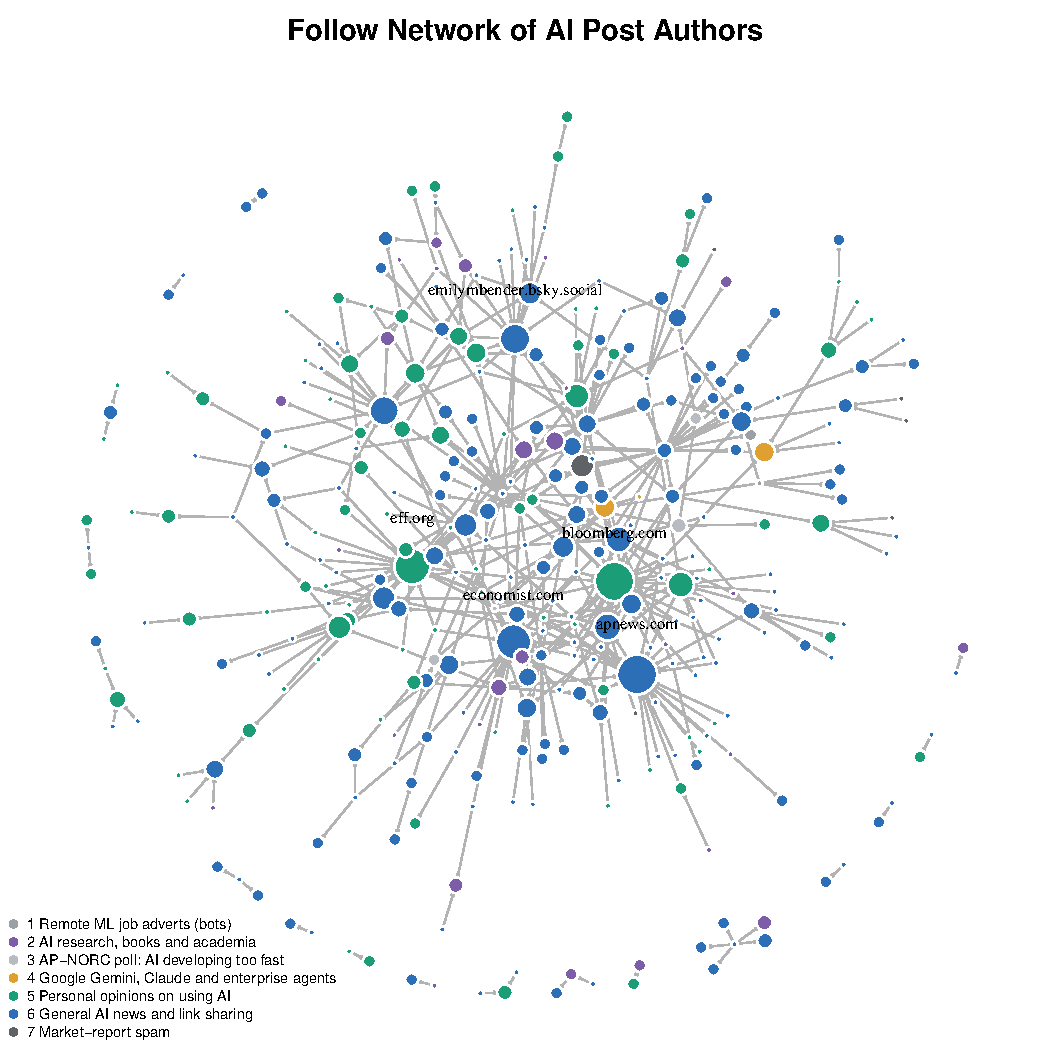
\includegraphics{Group6_analytical_report_files/figure-latex/full-network-1} 

}

\caption{Full follow network of AI-post authors (authors with at least one tie).}\label{fig:full-network}
\end{figure}

\textbf{Subgraph.} As in Module 7, the subgraph keeps authors with
\textbf{degree greater than 1}. This removes 163 loosely attached
authors and shows the core of the community more clearly. Centrality is
still calculated on the full graph.

\begin{Shaded}
\begin{Highlighting}[]
\NormalTok{keep }\OtherTok{=} \FunctionTok{degree}\NormalTok{(g) }\SpecialCharTok{\textgreater{}} \DecValTok{1}
\NormalTok{g2 }\OtherTok{=} \FunctionTok{induced\_subgraph}\NormalTok{(g, }\FunctionTok{V}\NormalTok{(g)[keep])}
\FunctionTok{c}\NormalTok{(}\AttributeTok{nodes =} \FunctionTok{vcount}\NormalTok{(g2), }\AttributeTok{edges =} \FunctionTok{ecount}\NormalTok{(g2))}
\end{Highlighting}
\end{Shaded}

\begin{verbatim}
#> nodes edges 
#>   177   325
\end{verbatim}

\begin{Shaded}
\begin{Highlighting}[]
\NormalTok{labels2 }\OtherTok{=} \FunctionTok{ifelse}\NormalTok{(}\FunctionTok{V}\NormalTok{(g2)}\SpecialCharTok{$}\NormalTok{name }\SpecialCharTok{\%in\%}\NormalTok{ top5, }\FunctionTok{V}\NormalTok{(g2)}\SpecialCharTok{$}\NormalTok{name, }\ConstantTok{NA}\NormalTok{)}
\FunctionTok{par}\NormalTok{(}\AttributeTok{mar =} \FunctionTok{c}\NormalTok{(}\DecValTok{0}\NormalTok{, }\DecValTok{0}\NormalTok{, }\DecValTok{2}\NormalTok{, }\DecValTok{0}\NormalTok{))}
\FunctionTok{set.seed}\NormalTok{(}\DecValTok{3020}\NormalTok{)}
\FunctionTok{plot}\NormalTok{(g2, }\AttributeTok{layout =} \FunctionTok{layout\_with\_kk}\NormalTok{(g2),}
     \AttributeTok{vertex.size =} \DecValTok{2} \SpecialCharTok{+} \FunctionTok{sqrt}\NormalTok{(}\FunctionTok{degree}\NormalTok{(g2, }\AttributeTok{mode =} \StringTok{"in"}\NormalTok{)) }\SpecialCharTok{*} \FloatTok{1.5}\NormalTok{,}
     \AttributeTok{vertex.color =}\NormalTok{ cluster.colours[author.cluster[keep]], }\AttributeTok{vertex.frame.color =} \StringTok{"white"}\NormalTok{,}
     \AttributeTok{vertex.label =}\NormalTok{ labels2, }\AttributeTok{vertex.label.cex =} \FloatTok{0.7}\NormalTok{, }\AttributeTok{vertex.label.color =} \StringTok{"black"}\NormalTok{,}
     \AttributeTok{vertex.label.dist =} \FloatTok{1.5}\NormalTok{, }\AttributeTok{vertex.label.degree =} \SpecialCharTok{{-}}\NormalTok{pi }\SpecialCharTok{/} \DecValTok{2}\NormalTok{,}
     \AttributeTok{edge.arrow.size =} \FloatTok{0.15}\NormalTok{, }\AttributeTok{edge.color =} \StringTok{"grey70"}\NormalTok{,}
     \AttributeTok{main =} \StringTok{"Authors with Degree \textgreater{} 1"}\NormalTok{)}
\FunctionTok{legend}\NormalTok{(}\StringTok{"bottomleft"}\NormalTok{, }\AttributeTok{legend =} \FunctionTok{paste}\NormalTok{(}\DecValTok{1}\SpecialCharTok{:}\DecValTok{7}\NormalTok{, cluster.names), }\AttributeTok{col =}\NormalTok{ cluster.colours,}
       \AttributeTok{pch =} \DecValTok{19}\NormalTok{, }\AttributeTok{cex =} \FloatTok{0.6}\NormalTok{, }\AttributeTok{bty =} \StringTok{"n"}\NormalTok{)}
\end{Highlighting}
\end{Shaded}

\begin{figure}

{\centering 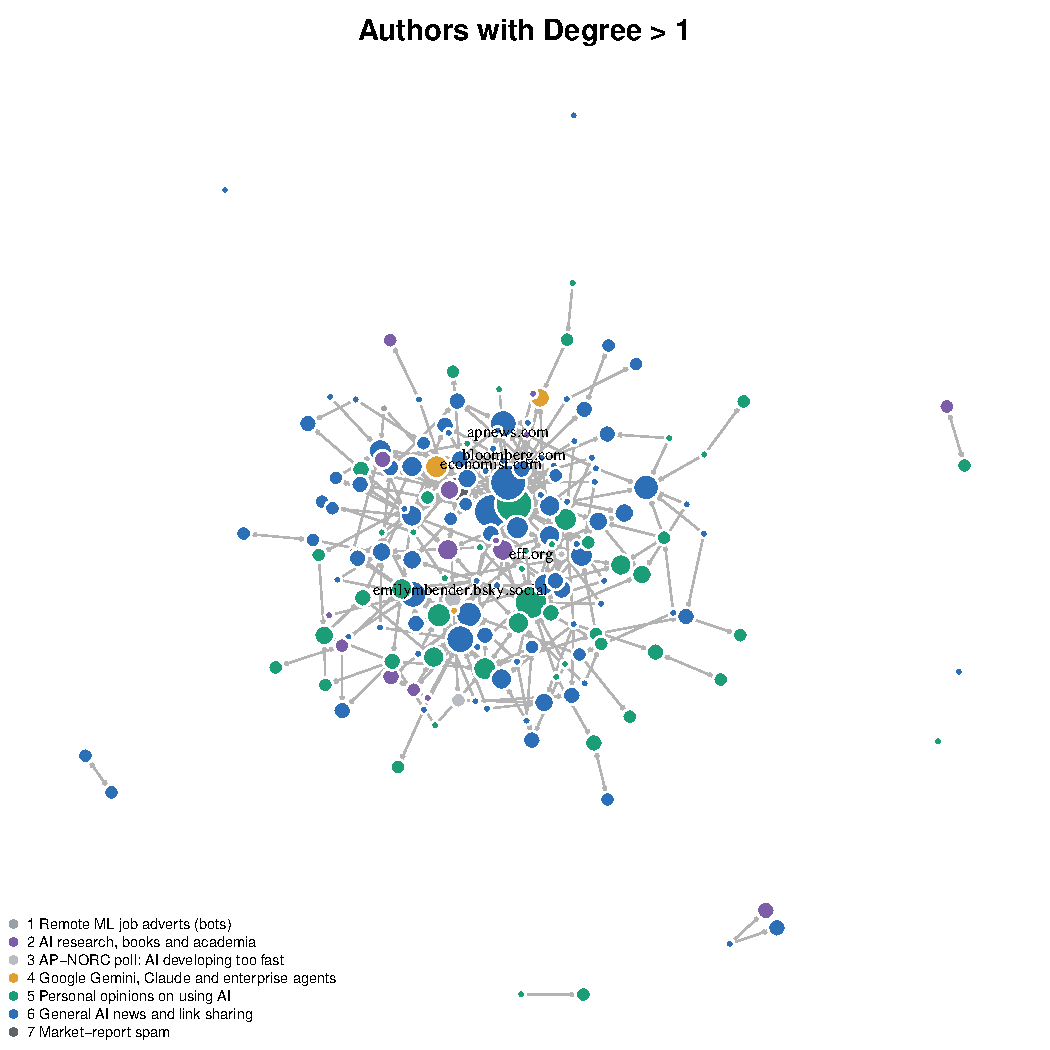
\includegraphics{Group6_analytical_report_files/figure-latex/subgraph-1} 

}

\caption{Subgraph of authors with degree greater than 1.}\label{fig:subgraph}
\end{figure}

\subsection{Centrality}\label{centrality}

Three centrality measures were calculated on the full graph:

\begin{itemize}
\tightlist
\item
  \textbf{In-degree:} the number of AI authors who follow the account
  (popularity).
\item
  \textbf{PageRank (Module 8):} an account is important if it is
  followed by other important accounts. As in the lab, the random surfer
  follows a link 80\% of the time (\texttt{damping\ =\ 0.8}).
\item
  \textbf{Betweenness:} how often an account lies on the shortest paths
  between other accounts (a possible bridge).
\end{itemize}

\begin{Shaded}
\begin{Highlighting}[]
\NormalTok{pr }\OtherTok{=} \FunctionTok{page\_rank}\NormalTok{(g, }\AttributeTok{damping =} \FloatTok{0.8}\NormalTok{)}\SpecialCharTok{$}\NormalTok{vector}
\NormalTok{btw }\OtherTok{=} \FunctionTok{betweenness}\NormalTok{(g, }\AttributeTok{directed =} \ConstantTok{TRUE}\NormalTok{)}

\NormalTok{top\_in }\OtherTok{=} \FunctionTok{head}\NormalTok{(}\FunctionTok{sort}\NormalTok{(in\_degree, }\AttributeTok{decreasing =} \ConstantTok{TRUE}\NormalTok{), }\DecValTok{5}\NormalTok{)}
\NormalTok{top\_pr }\OtherTok{=} \FunctionTok{head}\NormalTok{(}\FunctionTok{sort}\NormalTok{(pr, }\AttributeTok{decreasing =} \ConstantTok{TRUE}\NormalTok{), }\DecValTok{5}\NormalTok{)}
\NormalTok{top\_btw }\OtherTok{=} \FunctionTok{head}\NormalTok{(}\FunctionTok{sort}\NormalTok{(btw, }\AttributeTok{decreasing =} \ConstantTok{TRUE}\NormalTok{), }\DecValTok{5}\NormalTok{)}

\NormalTok{knitr}\SpecialCharTok{::}\FunctionTok{kable}\NormalTok{(}\FunctionTok{data.frame}\NormalTok{(}
  \AttributeTok{Rank =} \DecValTok{1}\SpecialCharTok{:}\DecValTok{5}\NormalTok{,}
  \AttributeTok{In\_degree =} \FunctionTok{paste0}\NormalTok{(}\FunctionTok{names}\NormalTok{(top\_in), }\StringTok{" ("}\NormalTok{, top\_in, }\StringTok{")"}\NormalTok{),}
  \AttributeTok{PageRank =} \FunctionTok{paste0}\NormalTok{(}\FunctionTok{names}\NormalTok{(top\_pr), }\StringTok{" ("}\NormalTok{, }\FunctionTok{round}\NormalTok{(top\_pr, }\DecValTok{3}\NormalTok{), }\StringTok{")"}\NormalTok{),}
  \AttributeTok{Betweenness =} \FunctionTok{paste0}\NormalTok{(}\FunctionTok{names}\NormalTok{(top\_btw), }\StringTok{" ("}\NormalTok{, }\FunctionTok{round}\NormalTok{(top\_btw), }\StringTok{")"}\NormalTok{)),}
  \AttributeTok{caption =} \StringTok{"Top five accounts for each centrality measure."}\NormalTok{)}
\end{Highlighting}
\end{Shaded}

\begin{longtable}[]{@{}
  >{\raggedleft\arraybackslash}p{(\linewidth - 6\tabcolsep) * \real{0.0472}}
  >{\raggedright\arraybackslash}p{(\linewidth - 6\tabcolsep) * \real{0.2830}}
  >{\raggedright\arraybackslash}p{(\linewidth - 6\tabcolsep) * \real{0.3585}}
  >{\raggedright\arraybackslash}p{(\linewidth - 6\tabcolsep) * \real{0.3113}}@{}}
\caption{Top five accounts for each centrality measure.}\tabularnewline
\toprule\noalign{}
\begin{minipage}[b]{\linewidth}\raggedleft
Rank
\end{minipage} & \begin{minipage}[b]{\linewidth}\raggedright
In\_degree
\end{minipage} & \begin{minipage}[b]{\linewidth}\raggedright
PageRank
\end{minipage} & \begin{minipage}[b]{\linewidth}\raggedright
Betweenness
\end{minipage} \\
\midrule\noalign{}
\endfirsthead
\toprule\noalign{}
\begin{minipage}[b]{\linewidth}\raggedleft
Rank
\end{minipage} & \begin{minipage}[b]{\linewidth}\raggedright
In\_degree
\end{minipage} & \begin{minipage}[b]{\linewidth}\raggedright
PageRank
\end{minipage} & \begin{minipage}[b]{\linewidth}\raggedright
Betweenness
\end{minipage} \\
\midrule\noalign{}
\endhead
\bottomrule\noalign{}
\endlastfoot
1 & apnews.com (26) & ketanjoshi.co (0.06) & vinkius-mcp-ai.bsky.social
(824) \\
2 & bloomberg.com (25) & nposegay.northsky.social (0.05) &
colin-fraser.net (620) \\
3 & eff.org (20) & savasavasava.myatproto.social (0.033) &
bigearthdata.ai (556) \\
4 & economist.com (19) & mattseybold.bsky.social (0.021) & bloomberg.com
(482) \\
5 & emilymbender.bsky.social (13) & apnews.com (0.019) &
pauljdavies.bsky.social (448) \\
\end{longtable}

\subsection{Interpretation}\label{interpretation-2}

\begin{itemize}
\tightlist
\item
  \textbf{In-degree} is led by news outlets (\textbf{apnews.com},
  \textbf{bloomberg.com}, \emph{economist.com}), the digital-rights
  organisation \emph{eff.org} and the AI-critical linguist
  \emph{emilymbender}. Within this sample, authors most often follow
  established organisations.
\item
  \textbf{PageRank} ranks a different set of accounts, mainly individual
  commentators (for example \textbf{ketanjoshi.co}). These accounts are
  followed by other well-connected authors, even if they are not
  followed by many authors overall.
\item
  \textbf{Betweenness} identifies bridges such as
  \textbf{vinkius-mcp-ai.bsky.social} and \textbf{colin-fraser.net},
  which connect otherwise separate parts of the network.
  \emph{bloomberg.com} is high in both in-degree and betweenness.
\item
  Most connected authors posted in the general news (207) or opinion
  (90) clusters. Very few authors from the automated clusters (job bots,
  market-report spam) are connected to other AI authors.
\item
  The three measures rank different accounts, so ``central'' depends on
  the definition: popular (in-degree), endorsed by important accounts
  (PageRank) or bridging (betweenness).
\end{itemize}

\subsection{Linking the network to engagement (RQ2 and
RQ3)}\label{linking-the-network-to-engagement-rq2-and-rq3}

RQ2 showed that engagement differs between topics. A natural follow-up
is whether it also differs with an author's position in the follow
network. We apply the same randomisation test (Module 10) to compare
posts by \textbf{connected authors} (at least one follow tie with
another AI author) and \textbf{isolated authors}.

\begin{itemize}
\tightlist
\item
  \textbf{H0:} mean engagement is equal for connected and isolated
  authors
\item
  \textbf{HA:} mean engagement differs (two-sided, \(\alpha = 0.05\))
\end{itemize}

\begin{Shaded}
\begin{Highlighting}[]
\NormalTok{connected }\OtherTok{=}\NormalTok{ posts}\SpecialCharTok{$}\NormalTok{author\_handle }\SpecialCharTok{\%in\%} \FunctionTok{V}\NormalTok{(g)}\SpecialCharTok{$}\NormalTok{name}
\NormalTok{isolatedEng }\OtherTok{=}\NormalTok{ posts}\SpecialCharTok{$}\NormalTok{engagement[}\SpecialCharTok{!}\NormalTok{connected]}
\NormalTok{connectedEng }\OtherTok{=}\NormalTok{ posts}\SpecialCharTok{$}\NormalTok{engagement[connected]}
\FunctionTok{c}\NormalTok{(}\AttributeTok{n\_isolated =} \FunctionTok{length}\NormalTok{(isolatedEng), }\AttributeTok{n\_connected =} \FunctionTok{length}\NormalTok{(connectedEng))}
\end{Highlighting}
\end{Shaded}

\begin{verbatim}
#>  n_isolated n_connected 
#>         581         450
\end{verbatim}

\begin{Shaded}
\begin{Highlighting}[]
\FunctionTok{c}\NormalTok{(}\AttributeTok{mean\_isolated =} \FunctionTok{mean}\NormalTok{(isolatedEng), }\AttributeTok{mean\_connected =} \FunctionTok{mean}\NormalTok{(connectedEng))}
\end{Highlighting}
\end{Shaded}

\begin{verbatim}
#>  mean_isolated mean_connected 
#>       1.500861       4.124444
\end{verbatim}

\begin{Shaded}
\begin{Highlighting}[]
\NormalTok{netDiff }\OtherTok{=} \FunctionTok{mean}\NormalTok{(connectedEng) }\SpecialCharTok{{-}} \FunctionTok{mean}\NormalTok{(isolatedEng)}
\FunctionTok{set.seed}\NormalTok{(}\DecValTok{123}\NormalTok{)}
\NormalTok{netDist }\OtherTok{=} \FunctionTok{replicate}\NormalTok{(}\DecValTok{1000}\NormalTok{, }\FunctionTok{shuffleMean}\NormalTok{(isolatedEng, connectedEng))}
\FunctionTok{hist}\NormalTok{(netDist, }\AttributeTok{col =} \StringTok{"lightblue"}\NormalTok{, }\AttributeTok{xlim =} \FunctionTok{range}\NormalTok{(}\FunctionTok{c}\NormalTok{(netDist, netDiff)),}
     \AttributeTok{main =} \StringTok{"Randomisation Distribution: Connected vs Isolated Authors"}\NormalTok{,}
     \AttributeTok{xlab =} \StringTok{"Difference in mean engagement (connected {-} isolated)"}\NormalTok{)}
\FunctionTok{abline}\NormalTok{(}\AttributeTok{v =}\NormalTok{ netDiff, }\AttributeTok{col =} \StringTok{"red"}\NormalTok{, }\AttributeTok{lwd =} \DecValTok{2}\NormalTok{)}
\end{Highlighting}
\end{Shaded}

\begin{figure}

{\centering 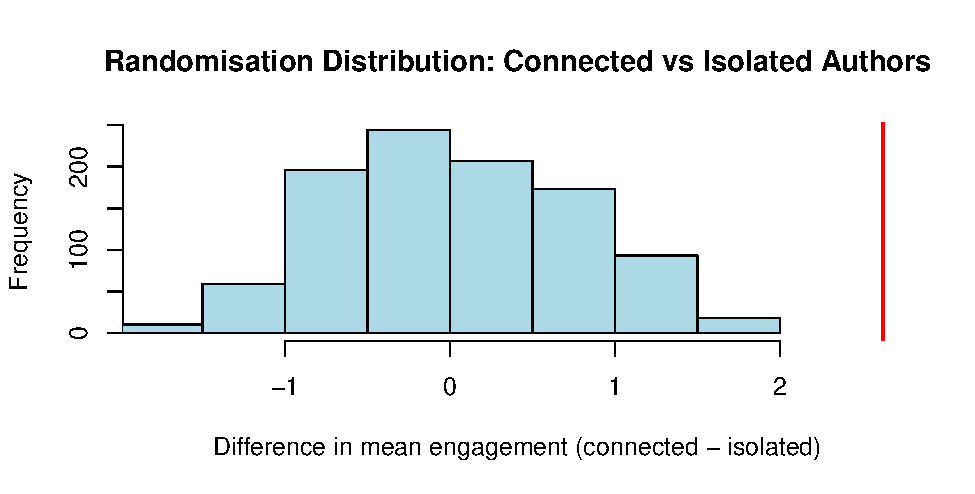
\includegraphics{Group6_analytical_report_files/figure-latex/network-engagement-1} 

}

\caption{Randomisation distribution for connected vs isolated authors; the red line is the observed difference.}\label{fig:network-engagement}
\end{figure}

\begin{Shaded}
\begin{Highlighting}[]
\NormalTok{netP }\OtherTok{=} \FunctionTok{mean}\NormalTok{(}\FunctionTok{abs}\NormalTok{(netDist) }\SpecialCharTok{\textgreater{}} \FunctionTok{abs}\NormalTok{(netDiff))}
\NormalTok{netP}
\end{Highlighting}
\end{Shaded}

\begin{verbatim}
#> [1] 0
\end{verbatim}

\begin{Shaded}
\begin{Highlighting}[]
\CommentTok{\# Among connected authors: followed by at least one other AI author?}
\NormalTok{followed }\OtherTok{=} \FunctionTok{names}\NormalTok{(in\_degree)[in\_degree }\SpecialCharTok{\textgreater{}} \DecValTok{0}\NormalTok{]}
\NormalTok{followedEng }\OtherTok{=}\NormalTok{ posts}\SpecialCharTok{$}\NormalTok{engagement[posts}\SpecialCharTok{$}\NormalTok{author\_handle }\SpecialCharTok{\%in\%}\NormalTok{ followed]}
\NormalTok{notFollowedEng }\OtherTok{=}\NormalTok{ posts}\SpecialCharTok{$}\NormalTok{engagement[connected }\SpecialCharTok{\&} \SpecialCharTok{!}\NormalTok{(posts}\SpecialCharTok{$}\NormalTok{author\_handle }\SpecialCharTok{\%in\%}\NormalTok{ followed)]}
\FunctionTok{c}\NormalTok{(}\AttributeTok{mean\_followed =} \FunctionTok{mean}\NormalTok{(followedEng), }\AttributeTok{mean\_not\_followed =} \FunctionTok{mean}\NormalTok{(notFollowedEng))}
\end{Highlighting}
\end{Shaded}

\begin{verbatim}
#>     mean_followed mean_not_followed 
#>          6.106464          1.336898
\end{verbatim}

Posts by connected authors received on average \textbf{4.12}
engagements, compared with \textbf{1.5} for isolated authors. None of
the 1,000 shuffled differences was as large as the observed difference
(p \textless{} 0.001), so \textbf{we reject H0}. Among connected
authors, those followed by at least one other AI author averaged 6.11
engagements, compared with 1.34 for those who follow others but are not
followed. This links the two analyses: \textbf{engagement is higher for
authors who are embedded in the AI community}. This is an association
within the sample, not evidence that follows cause engagement; for
example, active and established accounts may both attract followers and
receive more likes.

\subsection{Effect of data collection on the
network}\label{effect-of-data-collection-on-the-network}

\begin{itemize}
\tightlist
\item
  About 300 follows were collected per author. For authors who follow
  many accounts, some edges to other AI authors are missing, so missing
  follows may underestimate in-degree and distort betweenness.
\item
  The sample covers about one day of posts, so many authors in the AI
  community are not in the sample at all.
\item
  Keeping only follows between AI-post authors makes the network
  relevant to RQ3 but removes 463 authors with no ties from the graph.
\item
  A follow shows interest, not an actual conversation about AI.
\end{itemize}

\section{Overall Findings}\label{overall-findings}

\begin{enumerate}
\def\labelenumi{\arabic{enumi}.}
\tightlist
\item
  \textbf{What is discussed (RQ1):} AI discussion on Bluesky in this
  sample is dominated by \textbf{general AI news and link sharing} (57\%
  of posts) and \textbf{personal opinions about using AI} (25\%). A
  noticeable share is \textbf{automated or repeated content} (job bots,
  market-report spam, the same headline posted many times), which forms
  its own clusters.
\item
  \textbf{What gets engagement (RQ2):} opinion posts receive
  significantly more engagement than news posts (p = 0.032). Automated
  content receives almost no engagement. Across all seven topics, the
  one-way ANOVA did not find a significant difference.
\item
  \textbf{Who is connected (RQ3):} the authors form a \textbf{sparse}
  network. Most authors are not connected to each other, but the
  connected authors mainly form one large component. News outlets and
  organisations are the most followed accounts, while individual
  commentators rank highest on PageRank and betweenness. Automated
  accounts are almost absent from the connected core.
\item
  \textbf{How engagement and the network connect (RQ2 and RQ3):} posts
  by authors who are connected to other AI authors receive significantly
  more engagement than posts by isolated authors (p \textless{} 0.001),
  and authors followed by other AI authors receive the most.
\end{enumerate}

Together, the results suggest that, in this sample, \textbf{human
opinion posts about AI receive more engagement than shared news}. In the
follow network, authors most often follow established organisations,
while individual commentators occupy structurally central positions;
because the network is built from follows, it shows who pays attention
to whom, not where conversations take place. Engagement is concentrated
among authors who are embedded in the community, while automated
AI-related content makes up part of the volume but receives very little
engagement and is rarely connected to other authors.

\section{Limitations}\label{limitations}

\begin{itemize}
\tightlist
\item
  \textbf{Sampling:} keyword search over about 25 hours, sorted by
  latest. The results describe this sample, not all of Bluesky or all AI
  discussion.
\item
  \textbf{Text processing:} non-English posts lose most of their words
  after conversion to ASCII, and stemming produces shortened terms
  (e.g.~\emph{peopl}).
\item
  \textbf{Clustering:} there was no clear elbow, k-means depends on the
  chosen k and the random start (fixed with \texttt{set.seed}), and the
  two large clusters overlap.
\item
  \textbf{Hypothesis test:} engagement is very skewed with many zeros,
  and the t-test p-value is close to 0.05.
\item
  \textbf{Network:} limited follows per author, a sparse graph with 18
  components, and follows do not show actual interaction.
\end{itemize}

\section{References}\label{references}

\begin{itemize}
\tightlist
\item
  Gruber, J. B., Guinaudeau, B., \& Votta, F. (2024). \emph{atrrr:
  Wrapper for the AT Protocol behind Bluesky} {[}R package{]}.
  \url{https://CRAN.R-project.org/package=atrrr}
\item
  Feinerer, I., \& Hornik, K. (2024). \emph{tm: Text mining package}
  {[}R package{]}. \url{https://CRAN.R-project.org/package=tm}
\item
  Csardi, G., \& Nepusz, T. (2006). The igraph software package for
  complex network research. \emph{InterJournal, Complex Systems}, 1695.
\item
  Fellows, I. (2018). \emph{wordcloud: Word clouds} {[}R package{]}.
  \url{https://CRAN.R-project.org/package=wordcloud}
\item
  COMP3020 Social Web Analytics lab materials, Modules 4--10, Western
  Sydney University (2026).
\end{itemize}

\end{document}
